\documentclass[a4paper,11pt]{report}
\usepackage[T1]{fontenc}
\usepackage[utf8]{inputenc}
\usepackage{lmodern}
\usepackage[francais]{babel}
\usepackage{listings}
\usepackage[nottoc, notlof, notlot]{tocbibind}
\usepackage{rail}
\usepackage{graphicx}
\usepackage{listingsutf8}
\usepackage{float}
\usepackage[babel=true]{csquotes}
\usepackage[margin=2.5cm]{geometry}
\usepackage{longtable}

% Packages required by doxygen
\usepackage{fixltx2e}
\usepackage{calc}
\usepackage{doxygen}
\usepackage[export]{adjustbox} % also loads graphicx
\usepackage{graphicx}
\usepackage[utf8]{inputenc}
\usepackage{makeidx}
\usepackage{multicol}
\usepackage{multirow}
\PassOptionsToPackage{warn}{textcomp}
\usepackage{textcomp}
\usepackage[nointegrals]{wasysym}
\usepackage[table]{xcolor}

% Font selection
\usepackage{sectsty}
\newcommand{\+}{\discretionary{\mbox{\scriptsize$\hookleftarrow$}}{}{}}

% Hyperlinks (required, but should be loaded last)
\usepackage{ifpdf}
\ifpdf
  \usepackage[pdftex,pagebackref=true]{hyperref}
\else
  \usepackage[ps2pdf,pagebackref=true]{hyperref}
\fi
\hypersetup{%
  colorlinks=false,%
  linkcolor=blue,%
  citecolor=blue,%
  unicode%
}

% Custom commands
\newcommand{\clearemptydoublepage}{%
  \newpage{\pagestyle{empty}\cleardoublepage}%
}

\lstdefinelanguage{Stibbons}{
  morekeywords={
    new,agent,for,repeat,while,fd,forward,lt,turn-left,rt,turn-right,pd,pen-down,pu,pen-up,
    if,else,true,false,and,or,xor,not,function,null,null\_t,number\_t,boolean\_t,string\_t,
    color\_t,table\_t,turtle\_t,zone\_t,world\_t,send,recv,die
  },
  sensitive=false,
  morecomment=[s]{/*}{*/},
  morecomment=[l]{//},
  morestring=[b]',
  morestring=[b]",
}

\lstset{
  breaklines=true,
  captionpos=b,
  showstringspaces=true,
  tabsize=2,
  language=C++,
  frame=simple,
  float,
  floatplacement=H
}

\lstset{literate={'}{{'}}1 {"}{{\\"}}1 {é}{{\'e}}1 {è}{{\`e}}1 {ê}{{\^e}}1 {à}{{\`a}}1 {â}{{\^a}}1 {ç}{{\c{c}}}1 {Ç}{{\c{C}}}1}

\railalias{lbrace}{\{}
\railalias{rbrace}{\}}
\railalias{lpar}{(}
\railalias{rpar}{)}
\railalias{dot}{.}
\railalias{comma}{,}
\railalias{sharp}{\#}
\railalias{underscore}{\_}
\railalias{pipe}{|}
\railalias{ampersand}{\&}
\railalias{squote}{'}
\railalias{dquote}{"}
\railalias{tquote}{"""}
\railalias{nullt}{null\_t}
\railalias{numbert}{number\_t}
\railalias{booleant}{boolean\_t}
\railalias{stringt}{string\_t}
\railalias{colort}{color\_t}
\railalias{tablet}{table\_t}
\railalias{typet}{type\_t}
\railalias{turtlet}{turtle\_t}
\railalias{zonet}{zone\_t}
\railalias{worldt}{world\_t}
\railalias{turnleft}{turn\_left}
\railalias{turnright}{turn\_right}
\railalias{penup}{pen\_up}
\railalias{pendown}{pen\_down}
\railterm{lbrace,rbrace,lpar,rpar,dot,comma,sharp,underscore,pipe,ampersand,squote,dquote,tquote,nullt,stringt,numbert,booleant,colort,tablet,typet,turtlet,zonet,worldt,turnleft,turnright,penup,pendown}


%\author{Julia Bassoumi - julia.bassoumi@etud.univ-montp2.fr\\Florian Galinier - florian.galinier@etud.univ-montp2.fr\\Adrien Plazas - adrien.plazas@etud.univ-montp2.fr\\Clément Simon - clement.simon@etud.univ-montp2.fr}

\begin{document}

\title{Stibbons}

\makeatletter
  \begin{titlepage}
  \centering
        
\includegraphics[height=0.2\textheight]{doc/gestionProjet/stibbons.pdf}\\
        \vfill
        {\LARGE \textbf{\@title}}\\
        \vspace{1cm}
		{\large \textbf{\@date}}\\
		\vspace{1cm}
		{\large Julia Bassoumi - julia.bassoumi@etud.univ-montp2.fr\\Florian Galinier - florian.galinier@etud.univ-montp2.fr\\Adrien Plazas - adrien.plazas@etud.univ-montp2.fr\\Clément Simon - clement.simon@etud.univ-montp2.fr\\}
		\vspace{1cm}
		{\large Encadrant~: Michel Meynard}
        \vfill
        
\includegraphics[width=0.2\textwidth]{doc/gestionProjet/fds.png}
        \hfill
        
\includegraphics[width=0.2\textwidth]{doc/gestionProjet/UM2.png}
        \hfill
        
\includegraphics[width=0.2\textwidth]{doc/gestionProjet/depinfo.jpeg}
  \end{titlepage}
\makeatother

\begin{abstract}
Ce projet vise à la création d'un langage de programmation multi-agents pour programmeurs débutants et avancés, le Stibbons. Nous l'avons réalisé en C++ et ses applications utilisent le framework Qt.
Deux applications sont proposées pour répondre à deux cas d'utilisation différents~: une application graphique permettant de développer des programmes Stibbons et de les voir s'exécuter directement, et une application en ligne de commande simplifiant l'exécution d'un programme et permettant un export régulier de données du modèle exécuté.
Ce rapport expose le fonctionnement du langage Stibbons et de ses applications, ainsi que l'organisation que nous avons eu tout au long de la réalisation de ce projet.
\end{abstract}

\section*{Remerciements}
\phantomsection
Nous tenons tout particulièrement à remercier Michel Meynard pour avoir accepté de nous encadrer et pour son aide apportée tout au long du projet. Merci à lui de nous avoir accordé de son temps.

Nous souhaitions également remercier Jacques Ferber pour sa brillante introduction à la programmation multi-agents, ainsi que Sandrine Maton pour son aide apportée sur les méthodes agiles.

Le langage Stibbons tire son nom de la série de romans \emph{Les Annales du Disque-Monde} de Terry Pratchett.

\tableofcontents

\chapter{Introduction}
\section{Sujet}
	\subsection{Objectif}
	Le projet Stibbons est un projet visant à créer un interprète d'un dérivé de Logo, un langage de programmation permettant l'animation d'une «~tortue~» (cf \ref{Logo}). Nous avons choisi de développer un langage multi-agents, à l'instar de NetLogo ou StarLogo (cf \ref{NetLogo} et \ref{StarLogo}). Ainsi, l'objectif de ce projet était double~: la réalisation d'un interprète, capable d'analyser du code écrit dans un derivé de Logo, ainsi que la réalisation d'une application graphique capable de représenter l'évolution des agents.
	
	\subsection{Système multi-agents}
	Les systèmes multi-agents sont une approche de l'intelligence artificielle visant à facilité la résolution d'un problème en le découplant en plusieurs sous-problèmes. Ainsi, plutôt que de chercher à développer une intelligence unique complexe capable de résoudre le problème, l'approche multi-agent vise plutôt à créer des multitudes d'intelligences capables de résoudre qu'une petite partie du problème, et de compter sur l'intelligence collective émergeante pour voir apparaitre la solution au problème \cite{sma}.

	Ainsi, on peut prendre en exemple les fourmis qui, bien que n'ayant individuellement qu'une capacité «~limitée~», sont capables de survivre grâce à la synergie de leurs colonies.

\section{Cahier des charges}
	\subsection{Fonctionnalités attendues}
	Bien que la méthode de développement utilisée ai fait apparaitre de nombreuses fonctionnalités souhaitables au fur à mesure du projet, un certain nombre d'entre elles nous ont semblés indispensables dès le début~:
	\begin{itemize}
		\item chaque agent devait être capable de communiquer avec les autres agents~;
		\item chaque agent devait pouvoir modifier d'une certaine façon le monde~;
		\item des structures des langages modernes de la programmation impératives devaient être présent dans le langage (tels que les conditionnelles, les boucles, les fonctions, etc.)~;
		\item l'utilisateur devait pouvoir voir le monde où évoluent ces agents.
	\end{itemize}

        \subsection{Contraintes}
        Nous avions dès le début isolé un certain nombre de contraintes que nous voulions pour notre projet~:
        \begin{itemize}
          \item l'utilisation d'un langage non interprété, de type C ou C++~;
		  \item chaque agent devait évoluer parallèlement aux autres agents (threads)~;
          \item l'utilisation d'une méthode agile pour développer le projet.
        \end{itemize}


\chapter{Analyse de l'existant}
\section{Logo}
\label{Logo}

Le Logo est un langage apparu dans les années 60. Son objectif était de permettre à des personnes possédant peu de connaissances en informatique et en programmation (des enfants par exemple) de découvrir ce domaine de manière ludique et interactive. Ainsi, le langage permettait de diriger une tortue graphique, capable d'abaisser un crayon ou un feutre pour dessiner sur une feuille placé au sol. Les instructions entrées permettaient ainsi de tracer des formes, permettant une représentation très visuelle du code (la tortue physique est remplacé dans les implémentations moderne par une tortue virtuelle).

Le langage Logo en lui-même est un dérivé du Lisp (il est d'ailleurs parfois nommé Lisp sans parenthèses) et possède deux types de données~: les «~mots~» (chaîne de caractères) et les listes.

Du fait du public visé, les instructions de bases (par exemple \verb|forward|, \verb|left|, \verb|pendown|, etc.) et les structures du type procédures, boucles ou conditionnelles sont écrites de façon à être clairement explicite (cf. \ref{logo-proc}, \ref{logo-rpt} et \ref{logo-condi}).
Cependant, comme expliqué dans l'article \cite{Logo}, des études sur Logo ont montré que les enfants, hormis quelques exceptions, n'arrive pas à créer un programme entier et code «~ligne par ligne~» ce qui les empêchent de créer un modèle complexe et de cerner l'ensemble de la syntaxe de Logo.

\begin{lstlisting}[language=Stibbons,label=logo-proc,caption=Procédure en Logo]
to <nom de la procedure> :<parametre>
  <instructions>
  output <valeur a retourner>
end
\end{lstlisting}

\begin{lstlisting}[language=Stibbons,label=logo-rpt,caption=Boucle en Logo]
repeat <nb fois> [liste d'instruction]
\end{lstlisting}

\begin{lstlisting}[language=Stibbons,label=logo-condi,caption=Conditionnelles en Logo]
if <test> [liste d'instruction si vrai]
ifelse <test> [liste d'instruction si vrai] [liste d'instruction si faux]
\end{lstlisting}

Les instructions amènent la tortue à se déplacer, suivant une distance et un angle. On l'oriente ainsi suivant des coordonnées polaires.

\section{NetLogo}

NetLogo est un environnement de modélisation programmable pour simuler et observer des phénomènes naturels et sociaux au fil du temps. Il permet de donné des instructions et de regarder des agents réalisé ces dernières. On peut alors faire des observations et des connections inter-agents au niveau micro (individu par individu) comme au niveau macro (monde global).
NetLogo a été conçu pour des publics variés, notamment pour apprendre aux enfant à programmer, d'où sa syntaxe simple. Cependant, des études ont montré que les enfants, hormis quelques exceptions, n'arrive pas à créer un programme entier et code «~ligne par ligne~» ce qui les empêchent de créer un modèle complexe et de cerner l'ensemble de la syntaxe de NetLogo.
Il est aussi utilisé dans de nombreux domaines de recherche comme l'économie, la biologie, la physique,la chimie... et de nombreux articles ont été publié sur NetLogo.

Au niveau du programme en lui-même, NetLogo est composé de 3 onglets~: 
\begin{itemize}
	\item onglet info~: c'est la documentation du code~;
	\item onglet code~: le code permettant de crée le modèle du monde ainsi que le comportement des agents y sont implémentés. On peut y retrouver les différentes procédures ainsi qu'une procédure «~Mere~» qui permettra d'initialisé le modèle. Certaines procédures, ou parfois attributs, peuvent être lié à des widgets dans l'interface~;
	\item onglet interface~: l'interface contient deux parties.
\end{itemize}


La partie «~observation~» qui est représenté par une fenêtre où l'on verra notre modèle dans le temps.

La partie «~construction~» où l'on peut ajouter des widgets dans le but d’interagir avec le code. Par exemple un slider «~nb\_population~» qui permettra de choisir combien de tortue vont être crée sans modifier le code. On peut également y faire apparaître des boutons pour lancer on arrêter des procédures, des graphes pour observer des variations, des switch pour gérer les variables globales, des notes... On peut également contrôler le temps, ralentir pour mieux observer, accélérer pour voir ce que produit le modèle.


NetLogo permet donc une interaction très rapide entre le code et le rendu graphique. Ceci permet aux développeurs de «~jouer~» avec leurs modèles en modifiant facilement certaines conditions et donc d'ajuster immédiatement leur code comme ils le souhaitent.

Une riche documentation et de nombreux tutoriels est fourni sur le site officiel du langage, ce qui permet une prise en main simple et ludique.

NetLogo est un logiciel libre et open source, sous licence GPL. Il fonction sur la machine virtuelle Java, et est donc opérable sur de nombreuses plate-formes (Mac, Windows, Linux, etc.).
D'après le site officiel, NetLogo est décrit comme la prochaine génération de langage de modélisation multi-agents, tout comme StarLogo.



\section{StarLogo}
\label{StarLogo}
Tout comme NetLogo, StarLogo est un environnement de modélisation programmable pour simuler et observer des phénomènes naturels et sociaux au fil du temps.
Ils ont les mêmes objectifs d'études, d'éducations et de «~programmation facile~» ainsi qu'un aperçu direct du rendu (ref \cite{starlogo}).

Là où StarLogo diffère c'est qu'il n'est pas nécessaire de connaître une seule ligne de code. En effet, StarLogo se base sur un principe de bouton. Pour une partie de code donnée, un bouton y correspond. Les boutons peuvent être liées entre eux, ce qui permettra de créer des actions plus complexes.
Tout bouton peut être positionner dans une page, qui correspond aux différents «~environnements~» du modèle~: le monde globale, un certain type de tortue, les patchs, etc.
Par exemple, pour crée 12 tortues Turtles lors d'une initialisation globale du modèle il faut se positionner sur la page «~setup~», y placer les bouton «~setup~» attaché du bouton «~create Turtles - num~», puis modifier le «~num~» par 12.

StarLogo est composé de deux fenêtres~:
\begin{itemize}
  \item la fenêtre code~: c'est ici que les boutons sont placés dans les différentes pages pour généré le code.
  \item la fenêtre vue~: on y aperçoit le résultats du code généré. Le rendu peut être en 2D comme en 3D.
\end{itemize}

Au niveau historique, StarLogo avait d'abord été crée pour Mac lors de la première version, puis après plusieurs années, une version pour tout type d'environnement a vu le jour et la version uniquement pour Mac fut rebaptisé MacStarLogo. Plusieurs versions sont apparues mais c'est la version 2.1 de 2004 qui reste la plus récente.

Encore une fois, StarLogo obéit au même règles que son confrère~: c'est un logiciel libre sous licence GPL, il fonctionne sur la machine virtuelle Java d'où son regain de portabilité après la version MacStarLogo.


\chapter{Analyse des outils}
\section{Outils de gestion de projet}

\subsection{Méthodes agiles}

Pour réaliser ce projet, nous avons choisi de faire de l'Agile, avec la méthode SCRUM. Nous nous sommes principalement servi des cours de gestion de projet de ce semestre, en particulier des interventions de Sandrine Maton. Faire de l'Agile permet d'avoir un rendu fonctionnel à chaque fin de sprint, et donc de s'assurer d'avoir un rendu final. De plus, c'est une manière de faire qui se dévellope en entreprise, nous voulions donc l'expérimenter.
\subsubsection{Backlog}
Nous avons commencer le projet avec un sprint 0, au cours duquel nous avons défini l'univers du projet, et ses fonctionnalités (backlog). Voir ~\ref{backlogv1} page~\pageref{backlogv1}.


\begin{figure}[h]
\caption{\label{backlogv1} Backlog version 0.1}
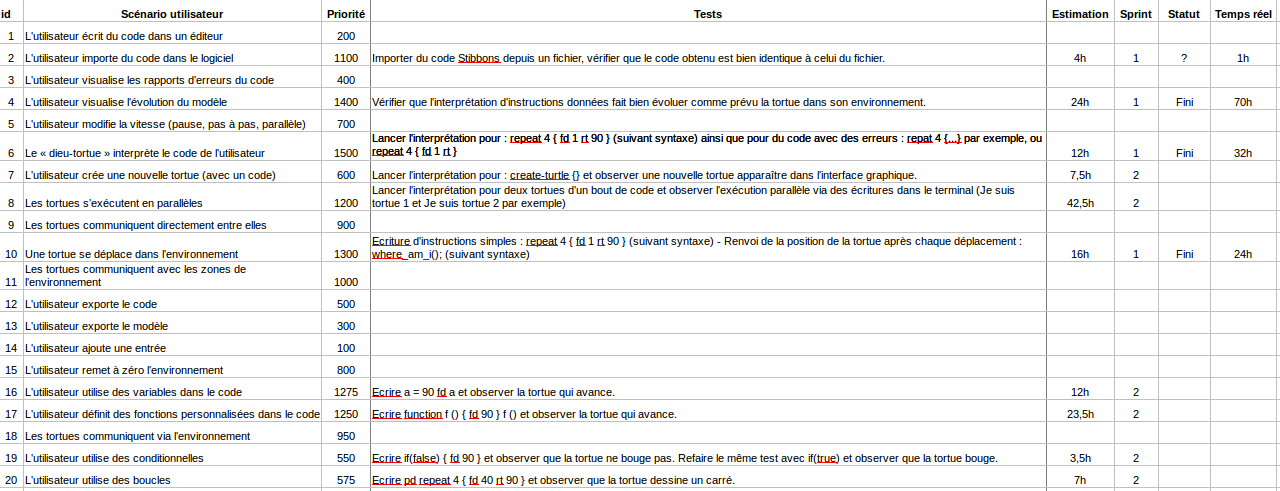
\includegraphics[scale=0.35]{doc/report/uml/backlogv1.png}
\end{figure}
Le backlog est composé de fonctionnalités, qui ont un indice entre 1000 et 0 pour leur importance du rendu final.

 On écrit aussi une \enquote{user-storie} pour chaque fonctionnalité. Cela correspond au test que l'on fait passer au programme pour valider la fonctionnalité.


A chaque sprint, on décide des fonctionnalités qu'on ajoute, et du nombre d'heures qu'on estime devoir y passer.


Voici pour comparer le backlog lors du début du sprint 4~\ref{backlogsp4} page~\pageref{backlogsp4} :


\begin{figure}[h]
\caption{\label{backlogsp4} Backlog sprint 4}
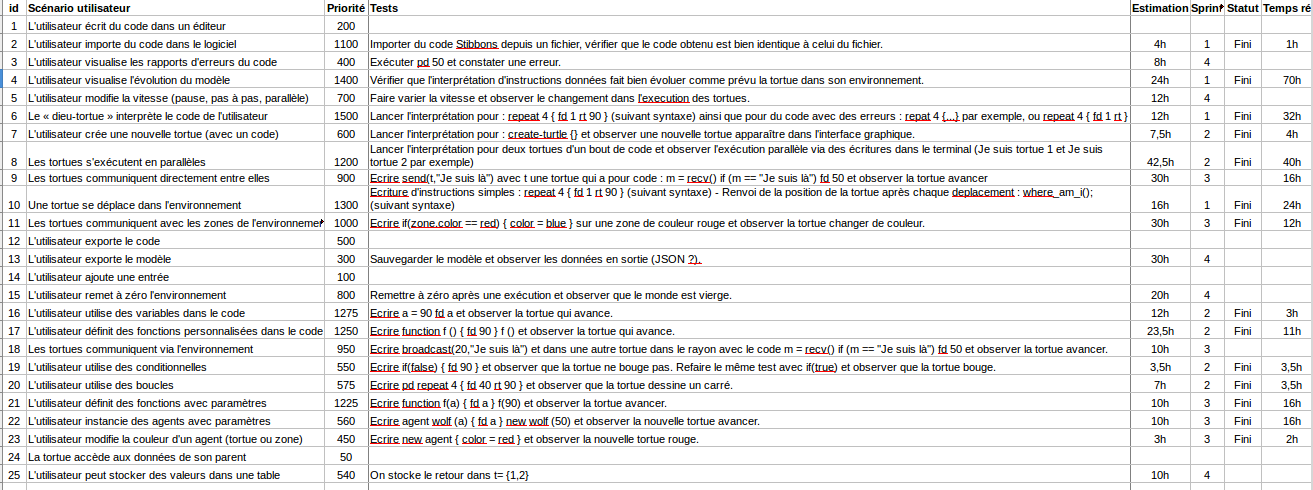
\includegraphics[scale=0.35]{doc/report/uml/backlogsp4.png}
\end{figure}
A la fin d'un sprint, on estime le temps passer sur chaque tâche, on fait le point sur notre avancée dans le projet.

Ici, on peut voir un ajout de fonctionnalités, le changement de statut des fonctionnalités réalisées, et le temps réel passer à les rendre utilisables.
Globalement, nous étions toujours dans les temps, car nous surestimions certaines tâches, qui s'averait plus facile que prévue.




\subsection{Git}
Git est hébergeur de code, de projet, qui permet d'avoir accès à ceux-ci n'importe où il y a internet.
Il s'utilise avec des systèmes de branches et s'utilise à la le plus souvent console, mais nous l'avons utiliser aussi avec Gitg, qui est une interface qui permet d'avoir un visuel des branches (Voir ~\ref{gitg} page~\pageref{gitg}).


\begin{figure}[h]
\caption{\label{gitg} Capture de Gitg}
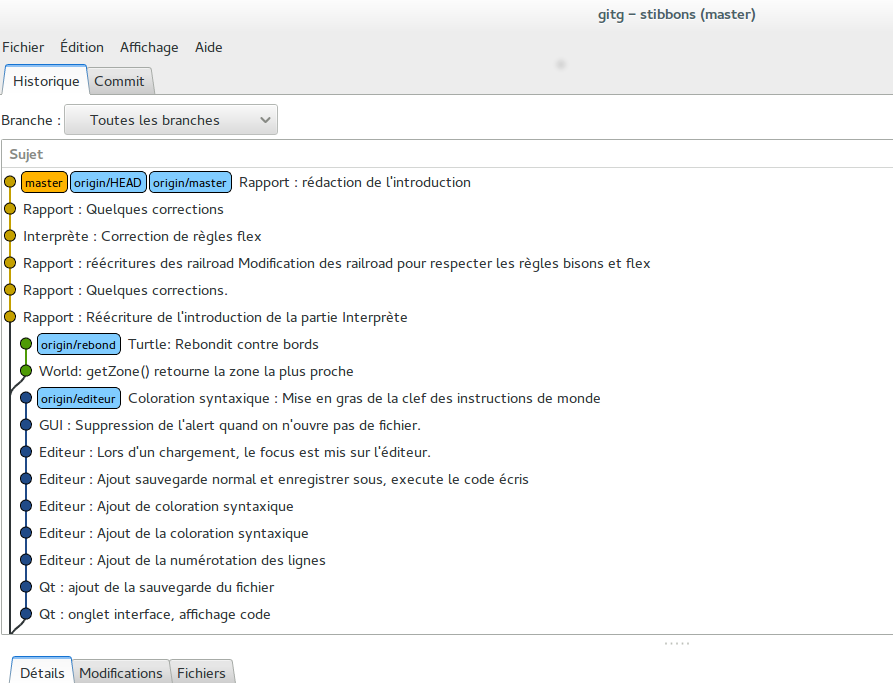
\includegraphics[scale=0.35]{doc/report/uml/gitbranche.png}
\end{figure}


Les commandes commence toujours par git :
\begin{itemize}
\item git checkout nom-branche, permet de changer de branche,
\item git branch, de savoir sur quel branche on est,
\item git add fichiers, permet de suivre des fichiers (enregistrer les modifications qu'on fait sur des fichiers),
\item git commit, permet de commiter les changements des fichiers qu'on suit,
\end{itemize}


De plus, Git permet sur son site de déclarer des \enquote{issues}. Ce sont des problèmes à corriger.



\subsection{Make}

Make est un utilitaire de construction de fichiers qui nous a été utile tout au long du projet pour construire les applications (stibbons et stibbons-cli), les tests unitaires, ou encore la documentation \LaTeX{} du projet. Il est également utile à l'installation des applications.

Il fonctionne en laissant l'utilisateur définir des règles de construction de fichiers en définissant les commandes nécessaires à celle-ci ainsi que les fichiers dont elle dépend.

Make est alors appelé à construire une cible (un fichier ou non), construisant son arbre de dépendances, vérifiant l'existance de ces dernières, les construisant ou reconstruisant au besoin. Ainsi Make permet d'éviter les compilations ou recompilations inutiles, accélerant et automatisant la construction de logiciels ou de documents.

\section{Tests unitaires}
\subsection{CppUnit}
CppUnit (ref.~\cite{CppUnit}) est un outil permettant d'organiser ses tests unitaires.
 On définit une classe de tests avec les attributs nécessaires aux tests, et des méthodes qui réalisent les tests souhaités. Cette classe est ensuite enregistrée dans le registre des tests pour être exécuter (cf. TestAgent.cpp).

CppUnit posséde des macros pour simplifier les tests comme :
CPPUNIT\_ASSERT(test), CPPUNIT\_ASSERT\_EQUAL(v1,v2),...

Lors de l'exécution, il indique combien de tests ont réussit et échoué.
Son écriture est simple, et son organisation permet une lecture rapide des tests.


\section{C++11}

\subsection{GDB}


\section{Outils d'analyse}

\subsection{Flex}
\label{Flex}

Flex est une version libre de l'analyseur lexical Lex (ref.~\cite{flex}). Il est généralement associé à l'analyseur syntaxique GNU Bison, la version GNU de Yacc.
Il lit les fichiers d'entrée donnés pour obtenir la description de l'analyseur à générer. La description est une liste de paires d'expressions rationnelles et de code C, appelées règles.

Un fichier flex est composé de plusieurs parties. La première contient une partie optionnelle de définition, encadrée par les symboles \verb|%{ %}| (cf. listing \ref{flex-definition}), ainsi que des options pour flex (cf. listing~\ref{flex-options}). La seconde partie est une partie obligatoire de règles, commençant par \verb|%%| (cf. listing~\ref{flex-regles}), tandis que la dernière partie est une nouvelle partie optionnelle, débutée par \verb|%%|, pouvant contenir des fonctions C/C++ définies par l'utilisateur (cf. listing~\ref{flex-fonctions}).

\begin{lstlisting}[caption=Partie définition d'un fichier flex,label=flex-definition]
%{
 int yyFlexLexer::yywrap() {
	return 1;
 }
%}
\end{lstlisting}

\begin{lstlisting}[caption=Options flex,label=flex-options]
%option c++
%option nodefault
\end{lstlisting}

\begin{lstlisting}[label=flex-regles,caption=Partie règles de flex]
%%
#([a-f0-9]{6}|[a-f0-9]{3}) {
							pyylval->v=make_shared<stibbons::Color>(yytext);
							return yy::parser::token::COLOR;
						   }
\end{lstlisting}
\begin{lstlisting}[label=flex-fonctions,caption=Partie fonctions de flex]
%%
int main(){
	// ...
}
\end{lstlisting}

La transformation en code C++ se fait par compilation via l'appel à l'application \verb|flex -+ exemple.l+|. La fonction d'analyse ainsi générée se nomme \verb|yylex()|.
Il faut par la suite penser à compiler le programme en liant la bibliothèque flex via le flag \verb|-lfl|.

\subsection{Bison}

GNU Bison est une version de yacc (ref.~\cite{bison}), un outil d'analyse syntaxique (cf.~\ref{analyse-syntaxique}). Il génère un analyseur syntaxique ascendant utilisant un automate à pile (dérivation à droite, on remplace le symbole non terminal le plus à droite).

Son fonctionnement est le suivant~: à chaque règle de grammaire, on associe des actions (instructions d'un langage). L'analyseur généré essaie de reconnaître un mot du langage défini par la grammaire. Il exécute les actions pour chaque règle reconnue.

Comme pour Flex, un fichier Bison est composé de trois parties. La première partie, facultative, contient une liste de définition C/C++, d'options bisons ainsi que de définition de jetons (cf. listing~\ref{bison-definition}), la seconde partie, contenue entre \verb|%%|, contient les règles (cf. listing~\ref{bison-regle}) et une dernière optionnelle de C/C++.

\begin{lstlisting}[label=bison-definition,caption=Definition C++ en bison]
%skeleton "lalr1.cc"
%defines
%locations
%parse-param { stibbons::FlexScanner &scanner }
%parse-param { stibbons::TreePtr t }
%parse-param { stibbons::TablePtr w }
%lex-param   { stibbons::FlexScanner &scanner }

%code requires {
	namespace stibbons {
		class FlexScanner;
	}

	std::string toString(const int& tok);
}

%token IF   "if"
%token ELSE "else"
%token FCT  "function"
\end{lstlisting}

\begin{lstlisting}[label=bison-regle,caption=Règles de grammaire en bison]
%%

//Storage of conditionnal expression
selection : IF expr statement
{
  stibbons::TreePtr t1 = make_shared<stibbons::Tree>(yy::parser::token::IF,nullptr);
  t1->addChild($2);
  t1->addChild($3);
  t1->setPosition({@1.begin.line,@1.begin.column});
  $$ = t1;
}
| IF expr statement ELSE statement
{
  stibbons::TreePtr t1 = make_shared<stibbons::Tree>(yy::parser::token::IF,nullptr);
  t1->addChild($2);
  t1->addChild($3);
  t1->addChild($5);
  t1->setPosition({@1.begin.line,@1.begin.column});
  $$ = t1;
};


%%
\end{lstlisting}

Les différents types de jeton sont déclarés via l'instruction \verb|%token NOM_DU_JETON| dans la première partie. On peut également définir le type C/C++ de la valeur du jeton via l'instruction \verb|%union|, ou en redéfinissant la macro \verb|YYSTYPE| (cf.~\ref{exemple-union} et \ref{exemple-yystype}).

\begin{lstlisting}[label=exemple-union,caption=Exemple du type des valeurs des jetons avant la 0.3]
%union{
  stibbons::Value* v;
  stibbons::Tree* tr;
}
\end{lstlisting}

\begin{lstlisting}[label=exemple-yystype,caption=Exemple du type des valeurs des jetons en 1.0]
#define YYSTYPE struct { stibbons::ValuePtr v; stibbons::TreePtr tr; int tok; }
\end{lstlisting}

Si on veut un analyseur syntaxique en C++, il faut utiliser un squelette de parseur C++ en utilisant soit l'option bison \verb|-skeleton=lalr1.cc|, soit en utilisant la directive \verb|%skeleton "lalr1.cc"|.

La transformation en code C++ se fait par compilation via l'appel à l'application \verb|bison -ydt exemple.y+|. La fonction d'analyse ainsi générée se nomme \verb|yyparse()| et fait appel en interne à \verb|yylex()|.

\section{Qt}

Qt est un framework d'application multi-plateformes écrit en C++ principalement utilisé pour la création d'interfaces graphiques.

\subsection{Multi plateforme et multi langages}

Qt est utilisable sur de nombreuses plateformes telles que Windows, Mac OS X, X11, Wayland, Android ou iOS.

De plus, bien que Qt soit développé en C++, ce n'est pas le seul langage depuis lequel il est utilisable, on trouve notament des liaisons pour Python, JavaScript, Go, Ruby, Haskell ou encore Ada.

\subsection{Modules}

Qt comprend de nombreux modules afin d'aider tant que possible le développement d'applications.
On peut particulièrement citer :
\begin{description}
	\item[Core]~: une implémentation des types de base (\verb|QString|, etc.), conteneurs, parallèlisme, entrées-sorties, système d'événements, etc.~;
	\item[Widgets]~: des widgets pour le développement d'interfaces graphiques~;
	\item[Network]~: support de divers protocoles réseau (TCP, UDP, HTTP, SSL, etc.)~;
	\item[Multimedia]~: lecture audio et vidéo~;
	\item[SQL]~: accès à des bases de données comprenant SQL~;
	\item[WebKit]~: moteur de rendu HTML~;
\end{description}

\subsection{Concepts fondamentaux}

\subsubsection{Widgets et layouts}

Qt propose un système de widgets complet et puissant. Il propose de nombreux widgets classiques tels que des boutons, des choix à puce, des onglets, des étiquettes, des images, etc.

Pour Qt, tout widget peut contenir des enfants et les arranger selon une disposition qui lui est affectée. Un widget n'ayant pas de widget parent sera considéré comme étant une fenêtre.
Son fonctionnement est ainsi assez différent de son concurrent Gtk+.

\subsubsection{Signaux et slots}

Qt propose également un système de signaux et de slots permettant d'implémenter le modèle observeur de manière efficace.

Ainsi un widget peut émettre des signaux contenant ou non des données (par exemple, pour signaler le changement de valeur d'une entrée) et un autre widget peut réceptionner ce signal dans un de ses slots, l'exécutant alors.

\subsubsection{Une extension à C++}

Qt propose une extension à C++~: il y ajoute des mots-clés pour permettre de simplifier la définition d'objets descendants de \verb|QObject|, tout particulièrement en spécifiant un ensemble de slots d'une certaine visibilité.
Ainsi lors de la déclaration d'une classe, il est possible de déclarer une liste de slots publics ou de signaux en les précédant des mentions \verb|public slots| et \verb|signals|, respectivement.
Le Meta-Object Compiler de Qt est alors utilisé pour convertir ces définitions en C++ classique à la compilation.

Qt propose également un système permettant d'embarquer des ressources (images, sons, etc.) directement dans le binaire produit via la définition d'un fichier de collection de ressources (\verb|.qrc|) et l'utilisation d'un Ressource Compiler.

qmake est un générateur de Makefiles permettant de simplifier l'utilisation du Meta-Object Compiler et du Ressource Compiler.

\subsection{Outils}

Qt permet de développer des interfaces dans un langage déclaratif basé sur XML. Pour utiliser ce puissant atout, il est conseillé d'utiliser Qt Designer, une application permettant de dessiner des interfaces graphiques de manière intuitive, en plaçant manuellement les widgets les uns dans les autres.

Qt Creator va encore plus loin puisqu'il est un IDE assez complet centré sur le développement d'applications avec Qt. En effet, il permet de gérer des projets, d'éditer du code, de concevoir des interfaces comme Qt Designer et même de créer des slots de manière graphique. Bien entendu il permet également de compiler, exécuter et débuguer le projet.

\subsection{Dessiner avec Qt}

Il est possible de réaliser des widgets personnalisés en redéfinissant la méthode \verb|paintEvent| d'un widget et en utilisant la classe \verb|QPainter| pour dessiner sur le widget.

Une instance \verb|QPainter| est liée à un widget et propose diverses méthodes permettant de dessiner~:
\begin{itemize}
	\item des lignes~;
	\item des arcs de cercle~;
	\item des polygones~;
	\item des ellipses~;
	\item des images~;
	\item du texte.
\end{itemize}


\section{Latex}

\subsection{Généralités}

\subsection{Beamer}


\section{JSON Spirit}
JSON Spirit (ref.~\cite{JsonSpirit}) est une librairie C++ qui permet de manipuler des fichiers JSON avec du C++.

Il utilise des structures de données C++ comme les vectors ou les maps, pour stocker les objets JSON. 

C'est un outil nouveau, mais assez puissant. Il n'est pas difficile à prendre en main : une classe \verb|Value| existe, et représente n'importe quels types de données (array, object, etc.) et sert de base pour la construction d'objet comme les \verb|Array| de JSON Spirit (un \verb|vector| de \verb|Value|), ou les \verb|Object| (un \verb|vector| de \verb|std::pair| C++).

Grâce à ces emboîtements, on peut représenter un fichier JSON exactement.


\chapter{Modèle}
\section{Sprint 1}
Lors du premier sprint, nous avons dû mettre en place la base du programme.\\ Pour le modèle, il s'agissait de mettre en place les classes :
\begin{itemize}
\item Turtle qui représente une tortue, 
\item Point, pour stocker les coordonnées d'une tortue,
\item Line, qui permettent aux tortues de laisser une trace (instruction pendown),
\item World.\\
\end{itemize}
Voir l'UML~\ref{v0.1} correspondant page~\pageref{v0.1}.\\
\begin{figure}[h]
\caption{\label{v0.1} UML de la version 0.1 prévue}
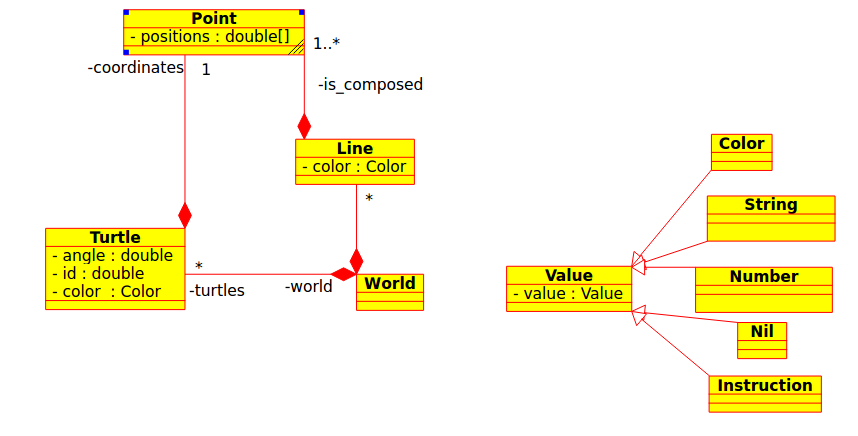
\includegraphics[scale=0.5]{doc/report/uml/v01.png}
\end{figure}
\newpage
La classe World représente le monde des tortues. Il contient la liste des tortues, et les lignes tracées par ces tortues.
Nous mettons aussi en place certains types Stibbons, comme Color, pour la couleur, ou Nil qui a une valeur nulle. Ils héritent de Value, une classe abstraite qui contient une valeur et ses accesseurs.\\

A la fin du premier sprint, nous avions réalisé ce schéma, en dehors de la classe Instruction qui n'était pas nécessaire. Les instructions tel que pendown, forward, etc... sont finalement des mots clés dans la grammaire du langage.\\
Voir figure~\ref{v0.1R} page~\pageref{v0.1R}.
\begin{figure}[h]
\caption{\label{v0.1R} UML de la version 0.1 réalisée}
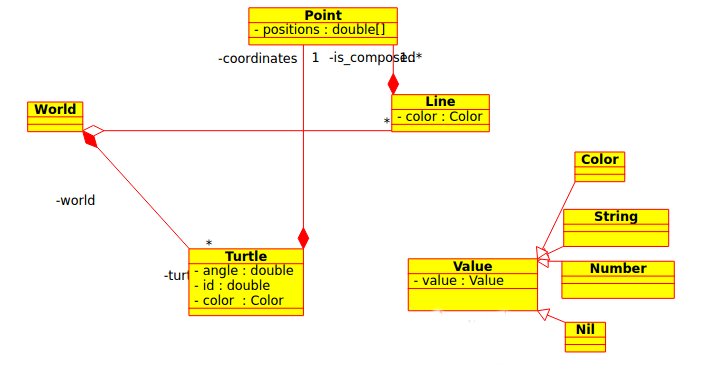
\includegraphics[scale=0.5]{doc/report/uml/v01reel.png}
\end{figure}
CAPTURE D'ECRAN DE L'APPLI

\section{Sprint 2}
Pour le second sprint, nous avons ajouté une classe Agent, car les classes World, Turtle et Zone sont des agents, au sens multi-agent.\\ Ils ont chacun un parent, celui qui l'a créer, une liste d'enfant, et des propriétés. Les propriétés sont des variables définit par l'utilisateur lors de la définition du code de l'agent, donc surtout utile pour les tortues.\\
Le monde a une taille, une liste de "breed", d'espèce. Il y a les espèces nommées et les "anonymes", qui sont des turtles dans le code.\\
Comme le montre ce code, on peut créer des tortues nommées ou pas.\\
METTRE UN EXEMPLE DE CODE DE L'UTILISATION DE BREED\\

Les types stibbons sont les mêmes, mais leurs définitions s'est un peu compléxifier en passant par une classe Simple-value, pour la mise en place des mutexs. Une énumeration des types Stibbons existe, elle est utiliser avec la méthode getType() pour pouvoir connaître le type de Value.\\
Pour que l'utilisateur puisse écrire des fonctions dans le code, nous avons ajouté une classe Function, qui stocke un arbre, qui contient le code la fonction, déja parser.\\
Le plus important, nous avons mis en place les threads dans l'interpreteur. Un nouveau thread correspond à une nouvelle tortue, c'est à dire, par rapport au code, à un "new agent".\\ Des mutexs ont été ajouté dans toutes les classes pour assurer que les threads sont thread-safe.\\
A la fin de ce sprint, nous devons relancer le programme pour charger un nouveau fichier de code, ce qui n'est pas pratique.\\
Voir figure~\ref{v0.2} page~\pageref{v0.2}.
\begin{figure}[h]
\caption{\label{v0.2} UML version 0.2}
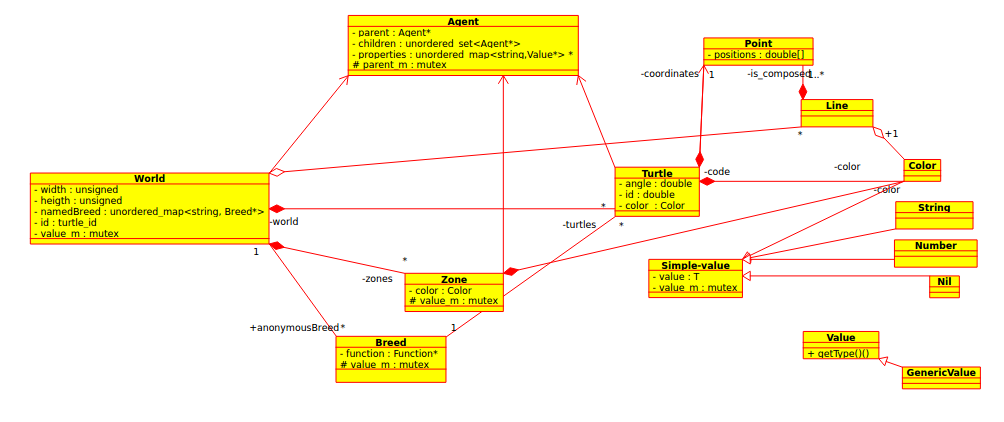
\includegraphics[scale=0.45]{doc/report/uml/v02reel.png}
\end{figure}
CAPTURE D'ECRAN DE L'APPLI
\newpage

\section{Sprint 3}

Lors du sprint 3, nous avons mis en place des pointers intelligents dans toutes nos classes REFERENCE A UN ARTICLE.\\
Nous avons ajouté des sous-classes de Function Standart-function et User-function pour représenter les fonctions standarts du langages. On les différencies des instructions par leurs parenthéses derrière leur nom.\\ Les user-function représentent les fonctions crées par l'utilisateur.\\
L'ajout de table fait aussi partit de ce sprint. Nous avons choisi, pour notre langage un seul type de conteneur : les tableaux.
Nous avons choisi de les écrire façon php, avec des accolades.\\
EXEMPLE DE CODE !!\\
Le but de ce sprint été la mise en place de la communication entre les agents. Les tortues peuvent "communiquer" avec les zones par écriture dans leurs propriétés. Les tortues peuvent communiquer entre elles grâce à des méthodes comme sendAll(message), recv(), etc...\\
Voir figure~\ref{v0.3} page~\pageref{v0.3}.
\begin{figure}[h]
\caption{\label{v0.3} UML version 0.3}
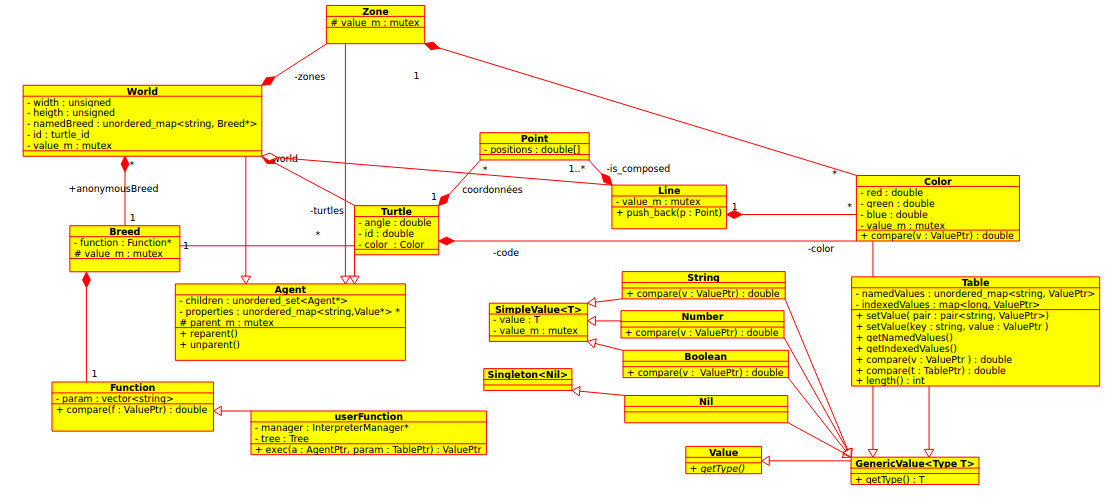
\includegraphics[scale=0.4]{doc/report/uml/v03.png}
\end{figure}
\section{Sprint 4}
Nous devons ajouter des fonctionnalités tel que la maitrise du temps et l'exportation du modèle. Ces ajouts ne provoque pas de changement du coté du modèle, si ce n'est quelques méthodes dans les classes World et Turtle et zone pour l'exportation du modèle.\\
L'exportation du modèle consiste à créer une sauvegarde de l'état du modèle à un instant t dans un fichier JSON.\\
Cela permettra ensuite, en passant par une transformation en CSV, d'avoir un tableau avec toutes ces données, ce qui permettra d'avoir des diagrammes de l'évolution du monde.\\

La maîtrise du temps se fait grâce à un bouton pause, qui arrête les threads qui s'executent, ou par un slider qui permet de ralentir ou de diminuer la vitesse. Cela se fait dans le code grâce à une méthode wait() qui fait lance sleep() sur le thread.\\

Le sprint 5 n'apporte pas de grand changement dans le modèle.



\chapter{Interprète}
L'application Stibbons fournit un interprète pour le langage du même nom. Cette interprétation du code se déroule en 2 phases~: une de compilation lors du chargement du code, et une d'interprétation de l'arbre abstrait généré lors de l'exécution.

La première phase peut elle-même être découpée en deux parties~:
\begin{itemize}
\item l'analyseur lexical qui «lit le flot de caractères qui constituent le programme source et les regroupe en séquences de caractères significatives appelées \emph{lexèmes}.» (\cite{compilateurs})~;
\item l'analyseur syntaxique qui, à partir des lexèmes, génère un arbre abstrait qui pourra par la suite être analysé pour être interprété.
\end{itemize}

L'interprétation quant à elle se déroule lors de l'analyse sémantique de l'arbre abstrait, qui exécute les opérations contenus par les nœuds.

\section{Analyseur lexical}
L'analyse lexicale vise à produire un flot de jetons qui pourront être analysés par l'analyseur syntaxique. Ces jetons sont des paires composées d'un type de jeton et de la valeur du lexème (par exemple, l'analyse du lexème \verb|12| va générer le jeton \verb|<NUMBER,12>| dans notre cas). Certains lexèmes peuvent générer des jetons qui n'ont pas de valeur (par exemple, le lexème \verb|(| va entraîner la génération du jeton \verb|<(>|).

Nous avons fait le choix d'utiliser l'outil Flex pour notre projet (cf.~\ref{Flex}).

\subsection{Jetons}
Notre analyseur lexical a dans un premier temps généré un nombre limité de jetons. Ainsi, en version 0.1, nous générions seulement 26 jetons différents (dont 5 jetons de littéraux), contre 40 jetons en version 1.0 (dont 7 jetons de littéraux). Ces jetons sont définis dans le code source bison (cf. listing~\ref{parser}) et leur valeur a un type C++ défini par la structure listing~\ref{struct-jeton}. Dans cette structure, l'attribut \verb|tok| correspond au type du jeton (défini par une énumération plus tard) tandis que l'attribut \verb|v| correspond à une valeur. En effet, notre langage ayant un typage dynamique, toutes les valeurs ont un type statique de type \verb|Value|. Ainsi, grâce au polymorphisme, le jeton aura une valeur qui pourra être de type dynamique \verb|Number|, \verb|String|, \verb|Boolean|, etc. tout en gardant un type statique de \verb|Value|. C'est lors de l'analyse sémantique (cf.~\ref{analyse-semantique}) que le type réel du jeton est analysé.

\begin{lstlisting}[label=struct-jeton,caption=Type des valeurs des jetons]
struct {
  stibbons::ValuePtr v;
  stibbons::TreePtr tr;
  int tok;
};
\end{lstlisting}

\subsection{Fonctionnement}
Par défaut, l'analyseur lexical généré par Flex utilise des variables globales et n'est pas réentrant. Dans l'optique d'obtenir un analyseur réentrant, nous avons utilisé l'option \verb|%option c++| et établit le modèle \ref{uml-lexer}.

\begin{figure}[h]
\centering
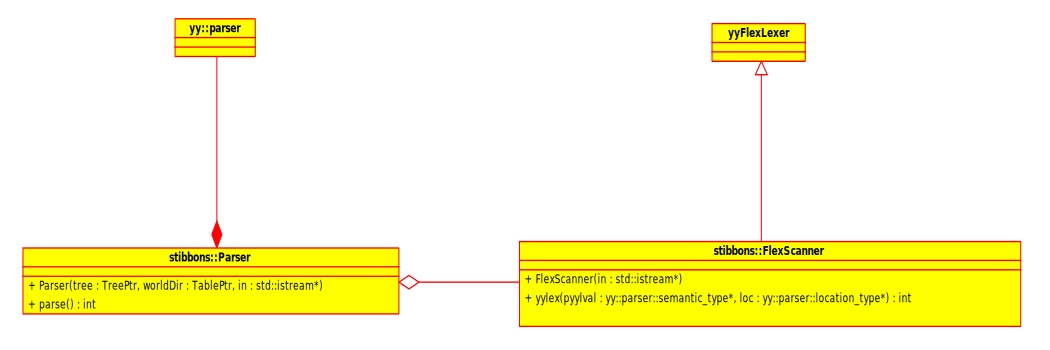
\includegraphics[scale=0.6]{doc/report/img/reentrant-parser}
\caption{\label{uml-lexer} UML des analyseurs lexical et syntaxique}
\end{figure}

Chaque appel à la méthode \verb|yylex()| de \verb|FlexScanner| génère un nouveau token à partir du flux d'entrée passé en paramètre lors de la construction de l'objet \verb|FlexScanner|. Cette méthode analyse le flux à partir des règles définies dans le fichier \verb|lexer.l+| (cf. listing~\ref{lexer}). Ainsi, les instructions définies pour chaque règle sont effectuées quand une chaîne de caractères correspondante à la règle est détectée. Ainsi, dans l'extrait \ref{lex-extrait}, lorsque l'analyseur détecte le caractère \verb|#| suivi d'une séquence de 3 ou 6 nombres hexadécimaux, l'appel au constructeur de \verb|Color(string)| est effectué. Ce dernier crée une couleur à partir d'une chaîne de caractère respectant les codes de couleur html.

\begin{lstlisting}[label=lex-extrait,caption=Exemple de séquence d'instruction lors de la détection d'une couleur]
#([a-f0-9]{6}|[a-f0-9]{3}) {
                           pyylval->v=make_shared<stibbons::Color>(yytext);
                           return yy::parser::token::COLOR;
                           }
\end{lstlisting}

De plus, l'instruction \verb|loc->step()| est effectuée au début de chaque appel à \verb|yylex()|, et permet de faire avancer la position actuelle de la longueur du lexème détecté, et l'instruction \verb|loc->lines()| est effectuée lors de la détection d'un retour à la ligne afin de faire avancer de \verb|n| lignes la position actuelle (avec \verb|n| le nombre de retour à la ligne détecté).
Les différentes règles flex peuvent être consultées au listing \ref{lexer}, ou de façon plus lisible dans l'annexe \ref{flex-rail}.


\section{Analyseur syntaxique}
L'analyse syntaxique permet de vérifier que la structure d'un programme est bien en accord avec les règles de grammaire du langage. Par exemple, la grammaire de notre langage comporte une règle, qui indique qu'un appel de fonction sans paramètre, est constituée du jeton \verb|<ID>| suivi des jetons \verb|<(>| et \verb|<)>|. Le but de notre analyse ici est double~: vérifier que le programme est bien un programme de notre langage valide, mais également générer un arbre abstrait qui pourra facilement être analysé par notre analyseur sémantique.

Nous avons fait le choix d'utiliser GNU Bison (cf.~\ref{Bison}) dans notre projet.

\subsection{Arbre abstrait}
Un arbre abstrait est une structure d'arbre dont chaque noeud feuille représente les opérandes des opérations contenues sur les autres noeuds. Cet arbre peut être considéré comme une forme de code intermédiaire, et peut être interprété très facilement en parcourant, pour chaque noeud, les sous-arbres et en appliquant l'opération du noeud courant.

\begin{figure}[h!]
\centering
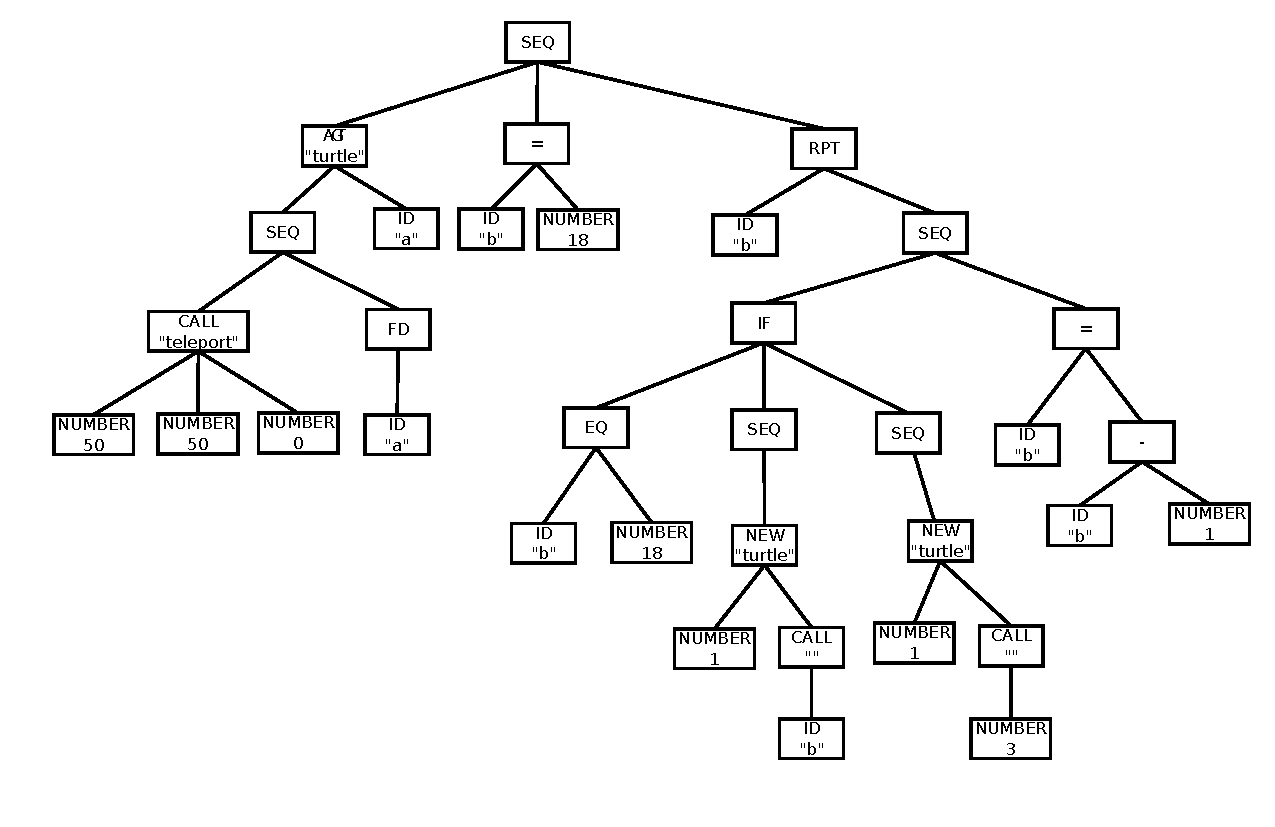
\includegraphics[scale=0.8]{doc/report/img/arbre-abstrait}
\caption{\label{arbre-abstrait} Arbre abstrait généré lors de l'analyse du code \ref{arbre-code}}
\end{figure}
\begin{lstlisting}[language=Stibbons,label=arbre-code,caption=Exemple de code Stibbons]
  agent turtle (a) {
    teleport(50,50,0)
    fd a
  }

  b = 18
  repeat b {
    if(b == 18) {
      new turtle(b)
    }
    else {
      new turtle(3)
    }
    b = b - 1
  }
\end{lstlisting}

L'avantage de générer un tel arbre est qu'il est bien plus rapide d'effectuer un parcours d'arbre à chaque interprétation plutôt que de refaire une analyse syntaxique à chaque fois.

\subsection{Fonctionnement}
L'écriture du fichier Bison est assez semblable au fichier Flex. En effet, on peut associer à chaque règle une liste d'instructions qui vont être exécutées lors de la détection de la règle. Ces instructions peuvent en outre être des affectations de valeur sémantique à une expression. Ainsi, dans l'extrait de code \ref{bison-extrait}, la valeur sémantique d'une sélection est un arbre dont les enfants sont dans l'ordre~: l'expression de test, la séquence d'instructions à exécuter si la condition est vrai et, optionnellement, la séquence d'instructions à exécuter si la condition est fausse.

\begin{lstlisting}[label=bison-extrait,caption=Cas du IF en Bison]
selection : IF expr statement 
{
  stibbons::TreePtr t1 = make_shared<stibbons::Tree>(yy::parser::token::IF,nullptr);
  t1->addChild($2);
  t1->addChild($3);
  t1->setPosition({@1.begin.line,@1.begin.column});
  $$ = t1;
}
| IF expr statement ELSE statement
{
  stibbons::TreePtr t1 = make_shared<stibbons::Tree>(yy::parser::token::IF,nullptr);
  t1->addChild($2);
  t1->addChild($3);
  t1->addChild($5);
  t1->setPosition({@1.begin.line,@1.begin.column});
  $$ = t1;
};
\end{lstlisting}

Bison génère à partir de ces règles un analyseur syntaxique LALR (\emph{look-ahead left-to-right rightmost derivation}). L'analyse du code et la génération de l'arbre sont lancées par un appel à la méthode \verb|stibbons::Parser::parse()| qui va elle-même faire appel à la méthode \verb|yy::parser::parse()|. L'ensemble du code va être analysé, cette méthode se chargeant de faire appel à la méthode \verb|stibbons::FlexScanner::yylex()|, générant et analysant les jetons en une seule passe.


\section{Analyseur semantique}
L'analyse sémantique du Stibbons est effectué dans les classes Interpreter. Plus exactement dans 3 classes. Voir l'UML~\ref{interpreterUML} correspondant page~\pageref{interpreterUML}.

\begin{figure}[h]
\caption{\label{interpreterUML} UML de l'analyseur sémantique}
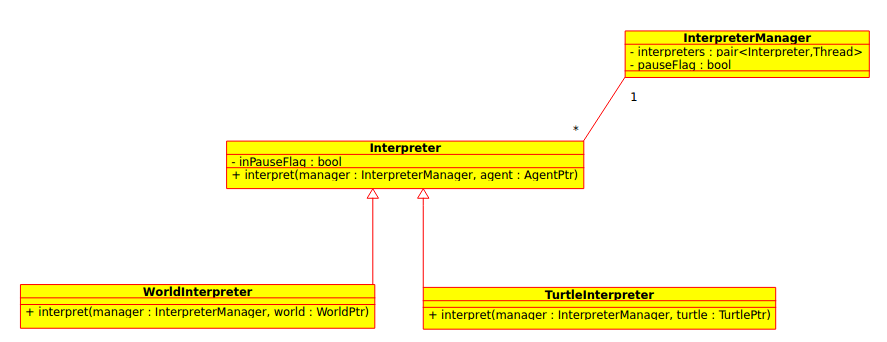
\includegraphics[scale=0.5]{doc/report/uml/interpreterUML.png}
\end{figure}

On a donc les classes \verb|TurtleInterpreter| et \verb|WorldInterpreter| qui héritent de la classe \verb|Interpreter|. Cette dernière analyse et provoque, dans le modèle, les actions liées au code stibbons écrit. Elle permet de gérer tout type d'interaction, du moment que ces actions ne sont pas liées à un monde ou une tortue. La classe \verb|TurtleInterpreter|, gère justement ce dernier type d'actions : celles liées à une tortue. Contrairement à \verb|WorldInterpreter| qui gère les actions du monde.

L'utilité de la classe \verb|InterpreterManager| est expliqué de manière détaillée dans la section \ref{remaniementInterpreter} (page~\pageref{remaniementInterpreter}).

Ainsi, pour avoir un exemple concret, si on demande à une tortue d'avancer en stibbons (ex : \verb|fd 10|), alors c'est le \verb|TurtleInterpreter| qui gèrera cette action.
A contrario, si on effectue une définition de fonction (ex : \verb|a = 10|) alors l'\verb|Interpreter| affectera la valeur \verb|10| à la propriété \verb|a| de l'agent courant.
Pour ce qui est du WorldInterpreter, il n'y a pas encore d'exemple possible, tout simplement car pour l'instant il n'y a pas d'actions spéciales pour le monde.

\subsection{Fonctionnalités}

\subsubsection{Sprint 1 \& 2}
Les deux premiers sprints ont été assez conséquent au niveau du nombre de fonctionnalités ajoutées.
En effet lors du sprint 1 on pouvait déjà effectuer les opérations de bases sur une tortue, telles que avancer, tourner, écrire, etc. De plus les opérations de calculs ainsi que la gestions de nombre ont été fait. En effet, il était nécessaire de gérer les nombres de manière à pouvoir indiquer à la tortue de quelle distance elle devait avancer.

Lors du deuxième sprint sont apparu les conditionnelles, ainsi que les boucles, les comparaisons binaires, les booléens et autres type (color, string, etc.), la création de nouveaux agents dans le code et les fonctions sans paramètres. Ce sprint fut alors une version déjà bien avancé de notre programme final.


\subsubsection{Sprint 3 à 5}
Les sprints suivants ont été plus léger. Non pas parce qu'il y avait moins de travail, car la gestion de l'interpréteur fut remanier à ce moment là, mais car il y avait moins de fonctionnalités à ajouter. En effet à partir du sprint 3, les fonctionnalités suivantes ont été rajoutés~:
\begin{itemize}
\item accès à la parenté et aux zones (en lecture seulement)~;
\item ajout des tables et de boucles dédiés (\verb|foreach|)~;
\item gestion de la vitesse et de la pause~;
\item ajout des communications avec le \verb|send| et le \verb|recv|.
\end{itemize}


\subsection{Remaniement de l'analyseur sémantique}
\label{remaniementInterpreter}

L'analyseur sémantique a d'abord été une seule classe~: la classe \verb|Interpreter|.
Cette dernière implémentait tout types d'actions a effectué pour n'importe quel type d'agent.
Cependant, lors de l'arrivé de la fonctionnalité d'ajout d'un nouvel agent (\verb|new agent|), nous nous sommes aperçu qu'il serait mieux d'avoir un interpréteur par type d'agent, ou plus précisement un interpréteur pour le monde, un pour les tortues et un pour les actions communes aux deux types.
Nous avons alors crée les deux classes~: \verb|WorldInterpreter| et \verb|TurtleInterpreter|.

De manière parallèle, la création du monde s'effectuait dans l'\verb|Interpreter|, puis dans le \verb|WorldInterpreter|, il fut alors nécessaire de crée une classe qui gérerait à la fois la création du monde et tout ce qui concernait l'application (la pause, le temps, les interpreteurs eux-mêmes). Nous avons alors décidé de crée la classe \verb|InterpreterManager|.
Cette classe connait ainsi tout les interpréteurs, permet de les prévenir d'une éventuelle pause du programme, de stocker les threads correspondants à chaque interpréteur, de crée un monde avec les pré-directives choisies~; c'est une sorte de gestionnaire d'interpréteurs.



\chapter{Applications}
\section{Application graphique}

\subsection{Version 0.1}

\begin{figure}[h]
\centering
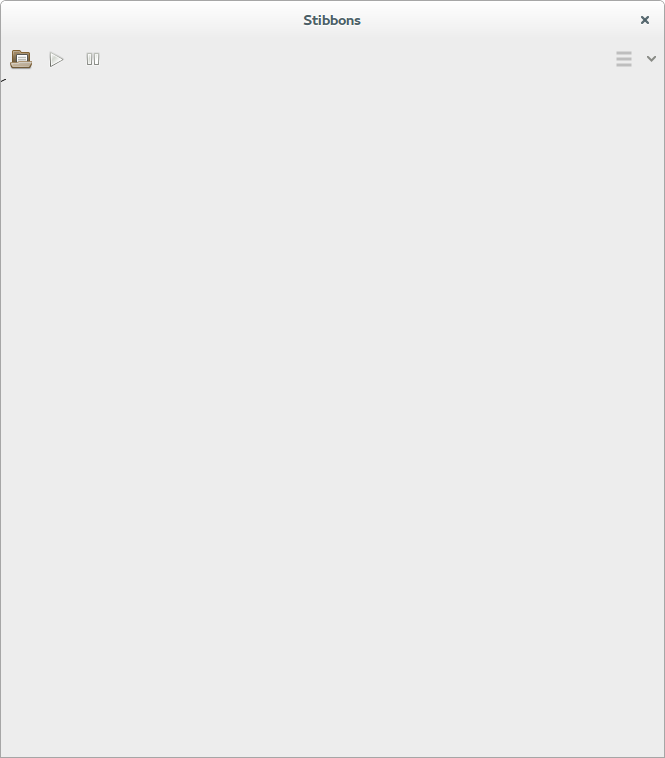
\includegraphics[scale=0.25]{doc/report/screenshot/stibbons-0-1-1.png}
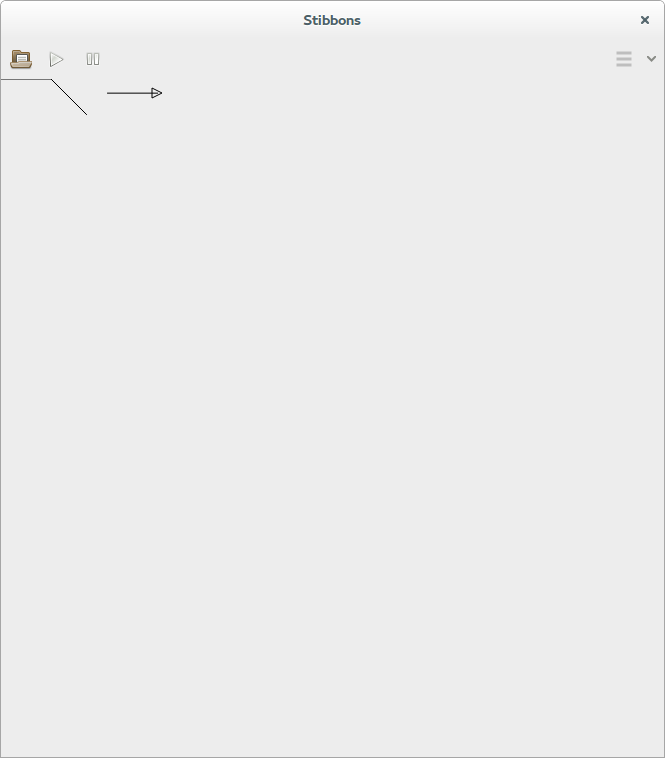
\includegraphics[scale=0.25]{doc/report/screenshot/stibbons-0-1-2.png}
\caption{\label{screenshot-0.1} Capture d'écran de la version 0.1}
\end{figure}

L'interface de la version 0.1 (cf. Figure~\ref{screenshot-0.1}) de Stibbons est composée d'une fenêtre séparée en une barre d'outil et une vue du monde.
La barre d'outil contient un bouton permettant d'ouvrir un fichier contenant un programme Stibbons (Ctrl+O), un bouton permettant d'exécuter le programme ouvert, un bouton de pause non fonctionnel, un bouton ouvrant un menu proposant la boîte de dialogues « À propos » et de quitter l'application (Ctrl+Q).

Si la boîte de dialogue permettant d'ouvrir un programme est fermée sans avoir choisi de fichier, une message d'erreur l'indiquant est alors affiché.

Une tortue existe par défaut dans le monde, elle est située dans le coin supérieur gauche de la vue et est orientée vers la droite. La tortue est alors dessinée comme un triangle noir creux et elle peut dessiner des lignes noires.

L'analyseur syntaxique n'étant alors pas réentrant, ouvrir plusieurs programmes les uns après les autres implique alors de redémarrer l'application.

\subsection{Version 0.2}

\begin{figure}[h]
\centering
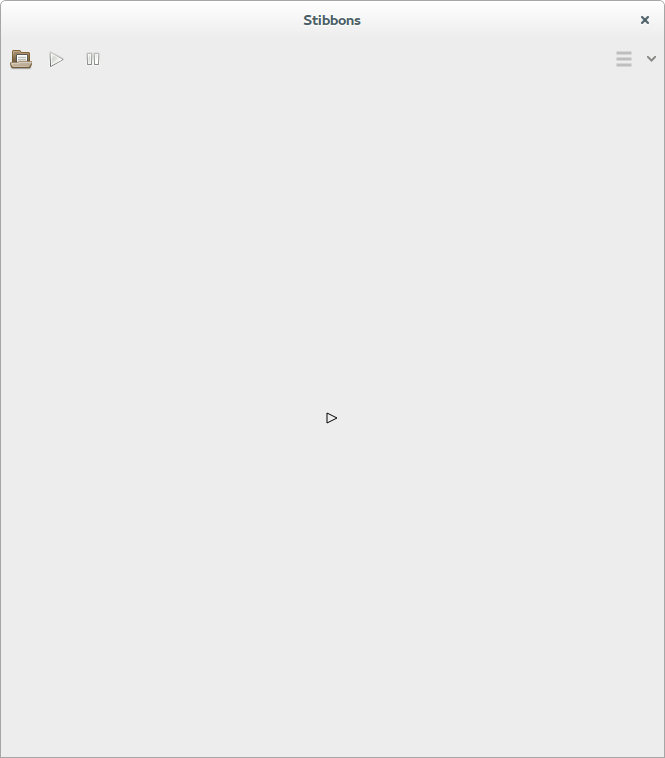
\includegraphics[scale=0.25]{doc/report/screenshot/stibbons-0-2-1.png}
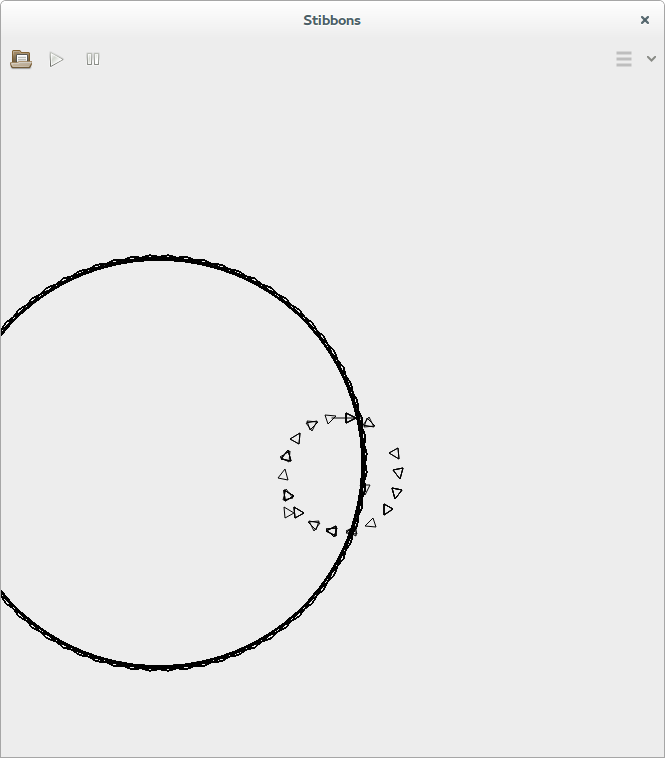
\includegraphics[scale=0.25]{doc/report/screenshot/stibbons-0-2-2.png}
\caption{\label{screenshot-0.2} Capture d'écran de la version 0.2}
\end{figure}

La version 0.2 (cf. Figure~\ref{screenshot-0.2}) apporte peu de modifications à l'application Stibbons elle-même, le changement le plus visible étant le placement temporaire de l'origine au centre de la vue, afin d'avoir une meilleure vue du programme s'exécutant.

\subsection{Version 0.3}

\begin{figure}[h]
\centering
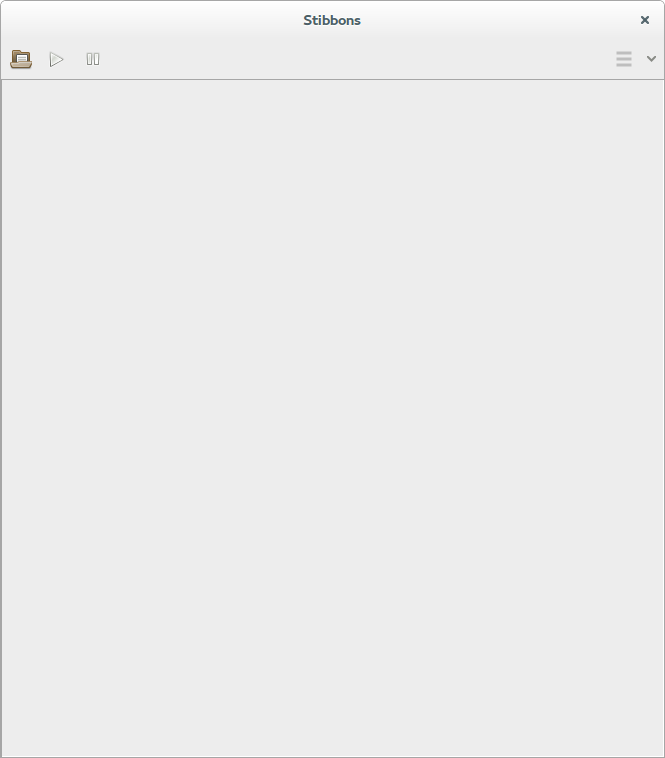
\includegraphics[scale=0.25]{doc/report/screenshot/stibbons-0-3-1.png}
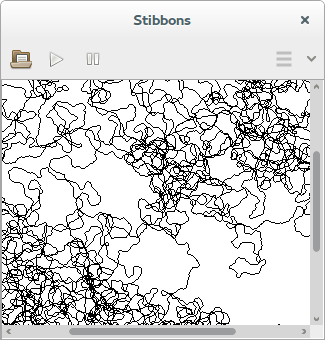
\includegraphics[scale=0.25]{doc/report/screenshot/stibbons-0-3-3.png}
\caption{\label{screenshot-0.3} Capture d'écran de la version 0.3}
\end{figure}

À partir de la version 0.3 (cf. Figure~\ref{screenshot-0.3}), les couleurs des tortues peuvent être modifiées et, afin de les rendre plus visibles, elles sont désormais dessinées comme des triangles pleins. La ligne dessinée par une tortue prend la couleur de cette dernière au moment de l'abaissement du stylo.

Le monde est désormais borné et est centré dans la vue, les zones le constituant sont désormais affichées, et leurs couleurs peuvent être modifiées. Si la vue est plus petite que le monde, des ascenseurs apparaissent.

Redessiner le monde prennait de plus en plus de temps au fur et à mesure que le nombre de lignes le constituant augmentait. Afin d'améliorer drastiquement ces performances de rendu, les lignes seront désormais dessinées sur un tampon et seules les nouvelles lignes auront donc besoin d'être dessinées sur ce dernier, avant d'être reporté sur la vue.

\subsection{Version 0.4}

\begin{figure}[h]
\centering
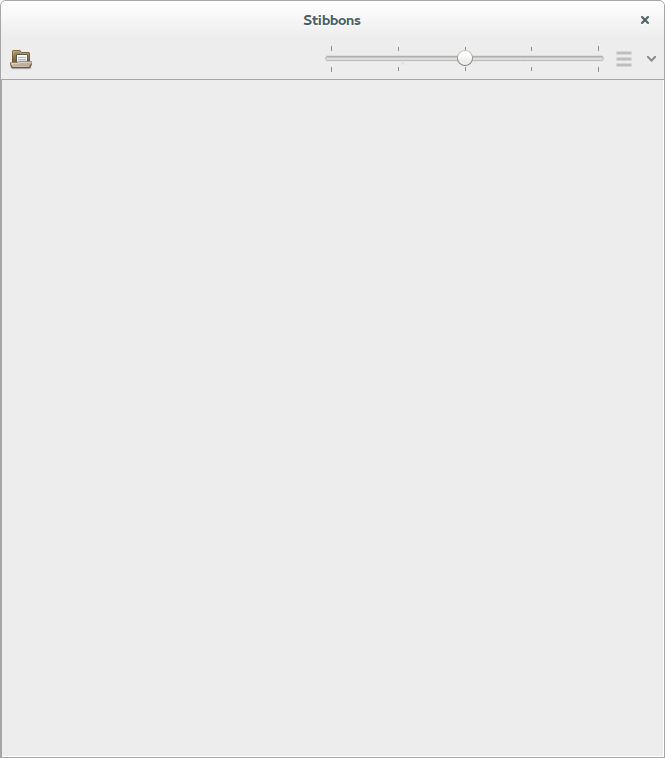
\includegraphics[scale=0.25]{doc/report/screenshot/stibbons-0-4-1.png}
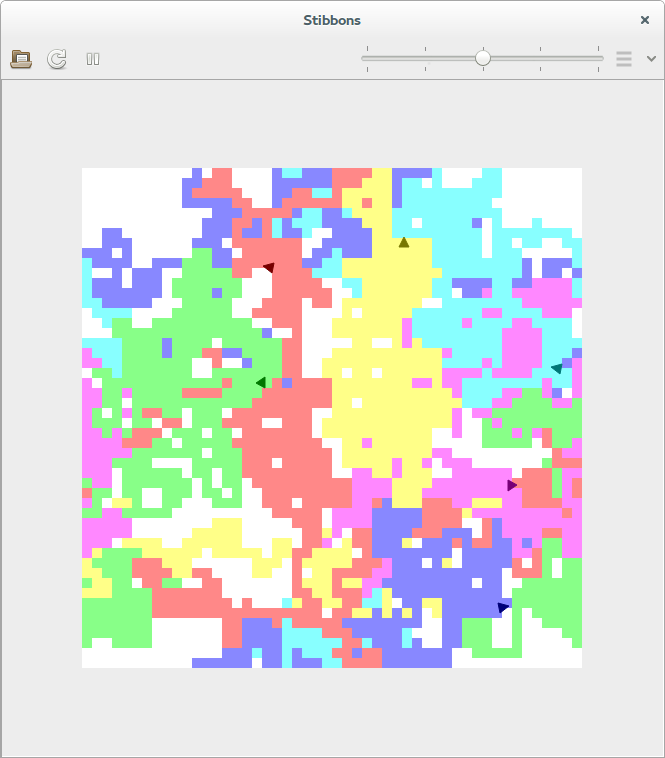
\includegraphics[scale=0.25]{doc/report/screenshot/stibbons-0-4-2.png}
\caption{\label{screenshot-0.4} Capture d'écran de la version 0.4}
\end{figure}

À partir de la version 0.4 (cf. Figure~\ref{screenshot-0.4}), il est possible de modifier la vitesse d'exécution du programme, de le mettre en pause, de reprendre son exécution et de le redémarrer depuis le début (F5). De plus, l'analyseur syntaxique étant désormais réentrant, il est possible d'ouvrir plusieur programmes les uns à la suite des autres.

Les boutons de démarrage et de mise en pause sont désormais confondus, et sont cachés, de même que le bouton de redémarrage, tant qu'aucun programme n'a été ouvert.

Une entrée a été ajoutée au menu, permettant d'exporter le modèle en cours d'exécution.

Si une tortue change de couleur alors qu'elle trace une ligne, le stylo avec lequel la tortue trace ses lignes changera de couleur en même temps.

Il est désormais possible de faire reboucler le monde sur lui même, cette option étant paramètrable pour chaque axe.

Le monde ne comporte plus de tortue par défaut et c'est désormais celui-ci qui exécute le corps principal du programme.

\subsection{Version 1.0}

\begin{figure}[h]
\centering
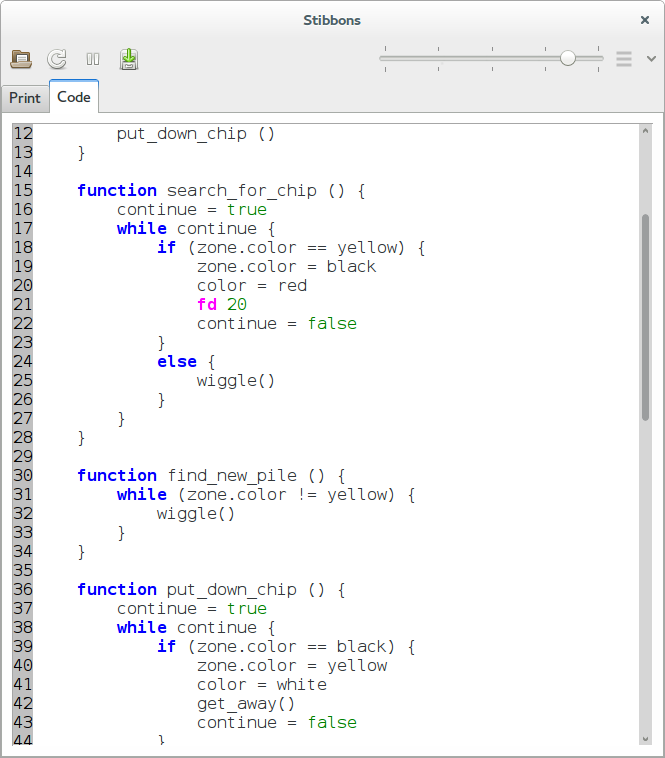
\includegraphics[scale=0.25]{doc/report/screenshot/stibbons-0-5-2.png}
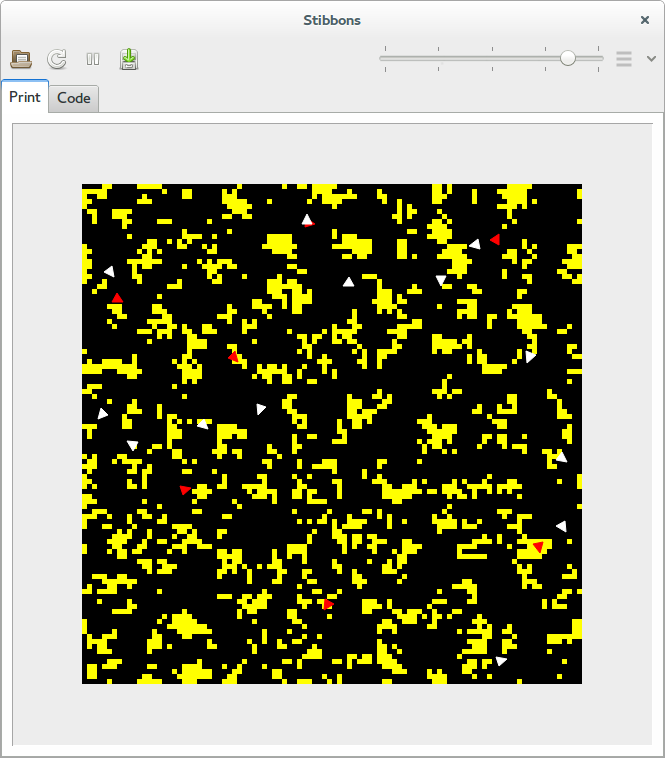
\includegraphics[scale=0.25]{doc/report/screenshot/stibbons-0-5-3.png}
\caption{\label{screenshot-1.0} Capture d'écran de la version 1.0}
\end{figure}

La version 1.0 (cf. Figure~\ref{screenshot-1.0}) marque l'apparition d'un éditeur de programme Stibbons dans l'application elle-même. L'éditeur propose également une coloration syntaxique. L'ajout de cet éditeur implique que les boutons de démarrage, de pause et de redémarrage ne soient plus cachés par défaut car il est désormais possible d'exécuter un programme écrit sans en avoir chargé un avant.

De nombreux raccourcis clavier sont ajoutés, afin d'enregistrer le programme dans son fichier (Ctrl+S) ou dans un nouveau fichier (Ctrl+Shift+S), d'exporter le modèle (Ctrl+E) et de démarrer ou mettre en pause l'exécution du programme (Ctrl+Espace).

Si la version 0.4 a ajouté une option permettant au monde de reboucler selon chaque axe, la version 1.0 permet d'avoir des bords solides, faisant rebondir toute tortue les croisant.

\section{Application en ligne de commande}

Une application en ligne de commande a été ajoutée à la version 0.4. Elle permet d'exécuter des programmes Stibbons sans serveur graphique et à pleine vitesse.

\subsection{Utilisation}

Utilisation~: stibbons-cli [options] fichier

Options~:
\begin{description}
	\item[-h, \texttt{-{}-}help] Affiche l'aide.
	\item[-v, \texttt{-{}-}version] Affiche l'information de version.
	\item[-e, \texttt{-{}-}export <secondes>] Exporte le modèle toutes les <secondes> secondes.
	\item[-p, \texttt{-{}-}prefix <prefixe>] Préfixe les fichiers exportés avec <prefixe>.
	\item[\texttt{-{}-}png] Génère une image PNG pour chaque export.
	\item[\texttt{-{}-}no-json] N'exporte pas le modèle dans un fichier JSON.
\end{description}

Arguments~:
\begin{description}
	\item[fichier] Le fichier de programme Stibbons à exécuter.
\end{description}

\subsection{Fonctionnement}

Le programme analyse la ligne de commande à l'aide de la classe QCommandLineParser, puis crée et exécute un objet représentant l'application selon les paramètres passés par l'utilisateur.

Lors de l'exécution de l'application, il est possible d'exporter le modèle à intervalle régulier grâce à l'option \texttt{-{}-}export. Par défaut, le modèle est exporté dans un fichier JSON, mais il est également possible d'exporter un rendu du monde en PNG, ou encore de ne rien exporter.

Afin de pouvoir dessiner le monde dans un fichier image, la classe WorldView, widget de l'application graphique jusque là responsable de dessiner le monde sur lui même, a vu ses fonctionnnalités de dessin d'un monde migrer vers la nouvelle classe WorldPainter, capable de dessiner un monde sur une surface.
Cette nouvelle classe est désormais utilisée dans l'application graphique par WorldView pour se dessiner, et par l'application en ligne de commande pour dessiner sur une QImage.


\chapter{Conclusion}
Durant quatre mois, nous avons réalisé ce projet que nous avions imaginé.
Ce projet a été positif à bien des égards. En effet, il nous a tout d'abord permis de pratiquer une méthode agile, ce qui était une bonne expérience et, avec le recul, un bon choix, car nous avions un projet fonctionnel toutes les deux semaines.
Nous avons pu en outre grâce à cette méthode ajouter facilement de nouvelles fonctionnalités en cours de route, avec notamment l'application en ligne de commande, complémentaire à notre programme principal.

Ce fut également une expérience profitable car nous avons pu voir l'importance de la communication sur ce type de développement. En effet, les cycles étant très courts, il était important de communiquer rapidement et clairement pour éviter de prendre du retard. Si nous avons parfois dépassé légèrement le délai (quelques heures de retard sur le premier sprint), nous avons tout de même sû gérer notre temps, ce qui nous a permis d'être dans les temps sur l'ensemble du projet.

Nous avons également pu grâce à ce projet travailler avec des outils nouveaux (Qt, JsonSpirit, \verb|std::thread|) et nous améliorer sur d'autres outils (Flex, Bison, Pointeurs intelligents).

Bien que la 1.0 soit une version fonctionnelle, il y a cependant des choses à améliorer. La première, et sans doute la plus importante, est le fait que notre parcours d'arbre se fait de façon récursive. Par conséquent, les appels récursifs en Stibbons vont impacter directement la pile d'exécution de l'interprète, et nous limite beaucoup.
De plus, les tortues évoluant chacune dans un thread séparé, on est relativement vite limité par le nombre de tortues pouvant évoluer dans notre programme (changement de contexte lourd).
Il y a également bon nombre de fonctionnalités que nous pourrions ajouter, comme les entrées dans l'interface, un peu à la manière de NetLogo, qui permettraient de modifier des propriétés de façon interactive avec l'exécution, ou encore l'affichage de la sortie standard dans un cadre du programme, voire dans des petites bulles au dessus des tortues.

Nous retiendrons néanmoins de notre projet un bilan positif. En effet, nous avons créé un langage, le Stibbons, ainsi que son interprète et une application graphique permettant de suivre l'évolution du modèle.


\listoffigures
\listoftables
\lstlistoflistings

\appendix

\chapter{Documentation}

\section{Syntaxe}

\subsection{Flex}
\label{flex-rail}
\begin{rail}
	ID : ( 'a-z' | underscore ) ( ( 'a-z'  | underscore | '0-9' ) * ) ;
	FD : 'fd' | 'forward'	;
	LT : 'lt' | 'turn-left'	;
	RT : 'rt' | 'turn-right' ;
	PD : 'pd' | 'pen-down' ;
	PU : 'pu' | 'pen-up' ;
	SEND : 'send'	;
	RECV : 'recv'	;
	DIE : 'die'	;
	AND : 'and' | ampersand ;
	OR : 'or' | pipe ;
	XOR : 'xor' | '\^{}' ;
	NOT : 'not' | '!'	;
	RPT : 'repeat' ;
	WHL : 'while' ;
	IF : 'if' ;
	ELSE : 'else' ;
	NEW : 'new' ;
	AGT : 'agent' ;
	FCT : 'function' ;
	FOR : 'for' ;
	IN : ':' | 'in' ;
	TYPE : nullt
	| numbert
	| booleant
	| stringt
	| colort
	| tablet
	| typet
	| turtlet
	| zonet
	| worldt
	;
	NIL : 'null' ;
	BOOLEAN : 'true' | 'false' ;
	STRING : squote ( WORD * ) squote
	| dquote ( WORD * ) dquote
	| tquote ( WORD * ) tquote
	;
	NUMBER : (('0-9' + ) ( (dot ( '0-9' * ) ) ?))
	| dot ( '0-9' + ) ;
	COLOR : sharp ('a-f' | '0-9') ('a-f' | '0-9') ('a-f' | '0-9') \\
	( ('a-f' | '0-9') ('a-f' | '0-9') ('a-f' | '0-9') ) ? ;
\end{rail}


\subsection{Bison}
\label{bison-rail}

\begin{rail}
code : worlddirlist statementlist | statementlist ;

worlddirlist : worlddir
| worlddirlist worlddir
;

worlddir : '\%' ID lit 'newline'
| 'newline'
;

statementlist : ( statement | statementlist statement ) ?
;

statement : exprstatement | complstatement;

complstatement : bloc
| declstatement
| selection
| loop
| complstatement 'newline'
;

bloc : lbrace rbrace
| lbrace statementlistbloc rbrace
;

statementlistbloc : statementlist
| statementlist exprnoseparator
;

declstatement : ( AGT | FCT ) ID lpar ( ( ID ( (',' ID) *) ) ? ) rpar bloc
;

selection : IF expr statement (ELSE statement) ? ;

loop : RPT expr statement
| WHL expr statement
| FOR (( lpar ( ID | ID ',' ID ) IN expr rpar ) | ((ID | ID ',' ID ) IN expr)) statement
;

exprstatement : 'newline'
| expr 'newline'
| instrturtle 'newline'
| creatstatement 'newline'
;

exprnoseparator : expr
| instrturtle
| creatstatement
;

expr : assignmentexpression
| lpar expr rpar
| expr ( '+'
| '-'
| '/'
| '*'
| '\%'
| AND
| OR
| XOR
| '=='
| '!='
| '>'
| '>='
| '<'
| '<=' ) expr
| '-' expr
| NOT expr
| primaryexpr
| lit
;

assignmentexpression : primaryexpr '=' expr
| primaryexpr '=' lbrace \\ (
(expr ((',' expr ) *))
| (expr ':' expr ((',' expr ':' expr ) *))
)? rbrace
;

primaryexpr : ID
| primaryexpr '.' ID
| primaryexpr '[' expr ']'
| primaryexpr '[' ']'
| ID lpar ( ( expr ((',' expr) *) ) ? )  rpar
;

creatstatement : (primaryexpr '=') ? \\ (NUMBER | primaryexpr)? (NEW AGT bloc
| NEW ID lpar \\ ( ( expr ((',' expr) *) ) ? ) rpar)
;

instrturtle : FD expr
| LT expr
| RT expr
| PU
| PD
| SEND expr expr
| SEND expr
| RECV primaryexpr primaryexpr
| RECV primaryexpr
| DIE ;

lit : NUMBER
| STRING
| BOOLEAN
| COLOR
| NIL
| TYPE ;
\end{rail}



\section{Propriétés standard}

Les agents possèdent certaines propriétés par défaut. Ces propriétés varient selon leur type, et peuvent être de simples attributs prédéfinis, des fonctions prédéfinies, ou encore des propriétés spéciales ayant une sémantique particulière.

Les propriétés spéciales ont une sémantique particulière et peuvent par conséquent être en lecture seule ou avoir certaines requêtes quant au valeurs qui lui sont affectées.

\subsection{Attributs communs aux tortues et au monde}

\begin{description}
	\item[black] $\rightarrow$ \#000000
	\item[white] $\rightarrow$ \#ffffff
	\item[grey] $\rightarrow$ \#7f7f7f
	\item[red] $\rightarrow$ \#ff0000
	\item[green] $\rightarrow$ \#00ff00
	\item[blue] $\rightarrow$ \#0000ff
	\item[yellow] $\rightarrow$ \#ffff00
	\item[cyan] $\rightarrow$ \#00ffff
	\item[magenta] $\rightarrow$ \#ff00ff
\end{description}

\subsection{Fonctions communes aux tortues et au monde}

\begin{description}
	\item[print] (value) $\rightarrow$ null

	Imprime une valeur sur la sortie standard.

	\begin{description}
		\item[value] La valeur à imprimer
		\item[Retourne] null
	\end{description}

	\item[println] (value) $\rightarrow$ null

	Imprime une valeur dans une nouvelle ligne sur la sortie standard.

	\begin{description}
		\item[value] La valeur à imprimer
		\item[Retourne] null
	\end{description}

	\item[rand] () $\rightarrow$ number

	Retourne un entier positif au hasard.

	\begin{description}
		\item[Retourne] un entier positif au hazard
	\end{description}
\end{description}

\subsection{Attributs du monde}

\begin{description}
	\item[max\_x] $\rightarrow$ number

	L'abscisse maximale du monde.

	\emph{Attribut en lecture seule.}

	\item[max\_y] $\rightarrow$ number

	L'ordonnée maximale du monde.

	\emph{Attribut en lecture seule.}
\end{description}

\subsection{Attributs des tortues}

\begin{description}
	\item[color] $\rightarrow$ \#000000

	La couleur de la tortue.

	\emph{Requiert une valeur de type color.}

	\item[parent] $\rightarrow$ agent

	L'agent qui a créé la tortue.

	\emph{Attribut en lecture seule.}

	\item[pos\_x] $\rightarrow$ number

	L'abscisse de la position de la tortue.

	\emph{Requiert une valeur de type number.}

	\item[pos\_y] $\rightarrow$ number

	L'ordonnée de la position de la tortue.

	\emph{Requiert une valeur de type number.}

	\item[pos\_angle] $\rightarrow$ number

	L'angle de la tortue.

	\emph{Requiert une valeur de type number.}

	\item[world] $\rightarrow$ world

	Le monde.

	\emph{Attribut en lecture seule.}

	\item[zone] $\rightarrow$ zone

	La zone dans laquelle est la tortue.

	\emph{Attribut en lecture seule.}
\end{description}

\subsection{Fonctions de tortues}

\begin{description}
	\item[distance\_to] (turtle) $\rightarrow$ number

	Retourne la distance la plus courte vers une autre tortue.

	\begin{description}
		\item[turtle] La tortue vers laquelle obtenir la distance
		\item[Retourne] null
	\end{description}

	\item[face] (turtle) $\rightarrow$ null

	Tourne la tortue pour qu'elle fasse face à une autre par le chemin le plus court.

	\begin{description}
		\item[turtle] La tortue à laquelle faire face
		\item[Retourne] null
	\end{description}

	\item[in\_radius] (distance) $\rightarrow$ table

	Retourne l' ensemble de tortues dans le rayon donné autour de la tortue.

	\begin{description}
		\item[distance] Le rayon autour de la tortue à sonder
		\item[Retourne] Une table contenant les tortues dans le rayon
	\end{description}

	\item[inbox] () $\rightarrow$ number

	Retourne le nombre de message non lus.

	\begin{description}
		\item[Retourne] Le nombre de messages non lus
	\end{description}

	\item[teleport] (x, y, angle) $\rightarrow$ null

	Téléporte une tortue à une certaine coordonnée et avec un certain angle.

	\begin{description}
		\item[x] L'abscisse où téléporter la tortue
		\item[y] L'ordonnée où téléporter la tortue
		\item[angle] L'angle à donner à la tortue
		\item[Retourne] null
	\end{description}
\end{description}

\subsection{Attributs des zones}

\begin{description}
	\item[color] $\rightarrow$ \#ffffff

	La couleur de la zone.

	\emph{Requiert une valeur de type color.}
\end{description}



\chapter{Tutoriel}

\section{Tutoriel}

\subsection{Salut, monde !}

Commençons par imprimer du texte.

\begin{lstlisting}[language=Stibbons]
println("Salut, monde !")
\end{lstlisting}

Ici l'agent par défaut, le monde, appelle la fonction println avec pour paramètre la chaîne de caractères "Salut, monde !", ce qui a pour effet d'imprimer ce texte dans une nouvelle ligne sur la sortie standard.

\subsection{Les premiers agents}

Créons maintenant des agents.

\begin{lstlisting}[language=Stibbons]
new agent {
    println("Salut, humain !")
}
\end{lstlisting}

Le monde crée un nouvel agent mobile, une tortue, qui apparaîtra alors dans le monde et exécutera le code passé entre accolades.

Il est possible de créer plusieur tortues exécutant le même code en spécifiant leur nombre.

\begin{lstlisting}[language=Stibbons]
5 new agent {
    println("Salut, humain !")
}
\end{lstlisting}

Ainsi, cinq tortues sont créés et chacune d'elles imprime "Salut, humain !".

\subsection{Dessiner un carré}

Les tortues peuvent se déplacer sur le monde en avançant et en tournant à gauche ou à droite. Elles ont également un stylo qu'elles peuvent abaisser ou relever afin de tracer des lignes sur le monde.

\begin{lstlisting}[language=Stibbons]
new agent {
    pd
    fd 50
    rt 90
    fd 50
    rt 90
    fd 50
    rt 90
    fd 50
    println("Voici un beau carré !")
}
\end{lstlisting}

Ici, pd demande à la tortue d'abaisser son stylo (pen down), fd demande à la tortue d'avancer (forward) d'une certaine distance, et rt demande à la tortue de tourner d'un certain nombre de degrés.

\subsection{Répéter}

Afin d'éviter de se répéter, on peut demander à l'interprète de le faire un certain nombre de fois pour nous.

\begin{lstlisting}[language=Stibbons]
new agent {
    pd
    repeat 4 {
        fd 50
        rt 90
    }
    println("Voici qui est mieux. =)")
}
\end{lstlisting}

\subsection{Boucler}

Il est également possible de boucler tant qu'une condition est vraie.

\begin{lstlisting}[language=Stibbons]
new agent {
    println("Je vais faire ma ronde.")
    while true {
        fd 50
        rt 90
    }
}
\end{lstlisting}

\subsection{Agents typés}

Il est possible de définir un type d'agent sans en créer, afin d'en créer plus tard.

\begin{lstlisting}[language=Stibbons]
agent personne (nom) {
    println("Je m'appelle " + nom + ".")
}

new personne("Mathieu")
new personne("Michel")
\end{lstlisting}

Ici, le type d'agent personne a été définit. Un type d'agent peut prendre des paramètres exactement de la même manière qu'une fonction.

Ainsi on a pu créer deux tortues de type personne, chacune ayant son propre nom.

\subsection{Fonctions}

Il est possible de définir des fontions. Les fonctions sont définies dans l'espace de nom des propriétés de l'agent.

\begin{lstlisting}[language=Stibbons]
%x_border bounce
%y_border bounce

agent fourmi () {
    function gigoter () {
        rt rand() % 60
        lt rand() % 60
        fd 1
    }

    while true {
        gigoter()
    }
}

new fourmi()
\end{lstlisting}

Les deux premières lignes seront expliquées un peu plus tard.

On définit ici la fonction gigoter pour les agents de type fourmi, qui est utilisée un peu plus bas dans le code.

\subsection{Couleurs}

Les tortues ont une couleur qui peut être modifiée. C'est également cette couleur qu'elles utilisent pour dessiner sur le monde.

\begin{lstlisting}[language=Stibbons]
%x_border bounce
%y_border bounce

agent fourmi (couleur) {
    function gigoter () {
        rt rand() % 60
        lt rand() % 60
        fd 1
    }

    color = couleur
    pd

    while true {
        gigoter()
    }
}

new fourmi(red)
new fourmi(blue)
\end{lstlisting}

\subsection{Propriétés d'autres agents et parent}

Il est possible d'accéder aux propriétés d'autres agents via l'opérateur «~\verb|.|~». De plus, il est possible d'accéder à certains agents via des propriétés spéciales, telles que \verb|parent| pour  obtenir le parent de l'agent actuel, \verb|world| pour obtenir le monde et \verb|zone| pour obtenir la zone sur lequelle se trouve une tortue.

Ces deux derniers types d'agents seront présentés un peu plus tard.

\begin{lstlisting}[language=Stibbons]
%x_border bounce
%y_border bounce

color = black

agent fourmi (enfants) {
    color = parent.color + #444

    if (enfants > 0) {
        2 new fourmi (enfants - 1)
    }

    function gigoter () {
        rt rand() % 60
        lt rand() % 60
        fd 1
    }

    while true {
        gigoter()
    }
}

new fourmi (2)
\end{lstlisting}

Dans cet exemple, chaque fourmi définit sa couleur en fonction de celle de son parent en l'obtenant via \verb|parent.color|.

\subsection{Le monde}

Le monde est un agent très particulier~: il est unique, immobile, possède une taille, et c'est dans son contexte qu'est exécuté le corps principal d'un programme Stibbons. Ça en fait de fait l'ancètre commun à tous les autres agents.

\begin{lstlisting}[language=Stibbons]
5 new agent {
    teleport(rand() % world.max_x, rand() % world.max_y, rand())
}
\end{lstlisting}

Cet exemple crée 5 nouveaux agents et, grâce aux fonctions \verb|teleport| et \verb|rand| et aux propriétés spéciales du monde \verb|max_x| et \verb|max_y|, positionne chaque agent une position et un angle au hazard à l'intérieur des bords du monde.

\subsection{Les zones}

Le monde est constitué de zones qui sont elles aussi des agents. Les zones sont immobiles, colorées, et ont le mond epour parent.

\begin{lstlisting}[language=Stibbons]
%x_border bounce
%y_border bounce

agent fourmi (couleur) {
    teleport(rand() % world.max_x, rand() % world.max_y, rand())

    function gigoter () {
        rt rand() % 60
        lt rand() % 60
        fd 1
    }

    color = couleur - #444
    couleur_zone = couleur + #888

    while (true) {
        gigoter()
        zone.color = couleur_zone
    }
}

new fourmi(red)
new fourmi(green)
new fourmi(blue)
new fourmi(yellow)
new fourmi(cyan)
new fourmi(magenta)
\end{lstlisting}

Ici, les fourmis changent la couleur des zones sur lesquelles elles passent.

\subsection{Directives de monde}

Dans cette section seront enfin expliquées les mystérieuses instructions \verb|%x_border bounce| et \verb|%y_border bounce|.

Le monde peut être paramétré au chargement du programme, pour cela on utilise des directives de monde qui doivent toutes être placées en tout début du programme.

Les directives \verb|%world_width| et \verb|%world_height| permettent de définir le nombre de zones constituant le monde en largeur et en hauteur, et doivent être suivi du nombre souhaité.
Les directives \verb|%zone_width| et \verb|%zone_height| permettent de définir la largeur et la hauteur des zones constituant le monde, et doivent être suivi de la taille souhaitée.
Les directives \verb|%x_border| et \verb|%y_border| permettent de définir le comportement des tortues lorsqu'elles franchissent un bord du monde. Elles doivent être suivies de \verb|none| pour laisser les tortues sortir du monde, de \verb|bounce| pour faire rebondir les tortues contre les bords ou de \verb|wrap| pour reboucler le monde sur lui même par l'axe en question.

\begin{lstlisting}[language=Stibbons]
%world_width 100  // Le monde aura 100 zones en largeur
%world_height 100 // Le monde aura 100 zones en hauteur
%zone_width 5     // Les zones feront 5 unités de large
%zone_height 5    // Les zones feront 5 unités de haut
%x_border wrap    // Le monde rebouclera sur lui même sur les bords verticaux
%y_border bounce  // Le monde sera solide sur les bords horizontaux
\end{lstlisting}

\subsection{Messages}

Les tortues peuvent s'envoyer des messages. Les messages peuvent être envoyés à un destinataire précis, à un ensemble de destinataires ou à toutes les tortues.

\begin{lstlisting}[language=Stibbons]
destinataire = new agent {
    recv message

    println("Quelqu'un m'a dit : " + message)
}

new agent {
    send "Coucou !" world.destinataire
}
\end{lstlisting}

\begin{lstlisting}[language=Stibbons]
5 new agent {
    recv message

    println("Quelqu'un m'a dit : " + message)
}

new agent {
    send "Oyez, agents !"
}
\end{lstlisting}

S'il n'y a aucun message dans sa boîte à messages, une tortue demandant la lecture d'un message sera bloquée jusqu'à réception d'un message à lire. Pour éviter un bloquage, il est possible de vérifier le nombre de messages présents dans la boîte.

\begin{lstlisting}[language=Stibbons]
new agent {
    new agent {
        send "Bonjour, parent !" parent
    }

    while true {
        if (inbox() > 0) {
            recv message

            println("Quelqu'un m'a dit : " + message)
        }

        rt 1
        fd 1
    }
}
\end{lstlisting}



\chapter{Résumés des réunions}

\section{27 janvier 2015}

Voici le résumé de la première réunion, le 27 janvier.\\
Tout d'abord,petite précision et chose à faire rapidement :
\begin{itemize}
\item  trouver un article à lire sur le multi-agents
\item le rapport sera fait en Latex
\item il faut créer un dêpot GIT du Sif pour mettre le travail et le rapport
\end{itemize}

Résumé du projet :\\
Nous allons développer un système multi-agent sur une même machine, pas de réseau.\\
Nous avons d'abord parler de faire un ordonnanceur de tâche pour exécuter les agents un à un, comme en NetLOGO, puis nous avons plutôt opter pour l’exécution en parallélisme des tortues, car faire un ordonnanceur causerai des difficultés, (comme comment récupérer la main sur les tortues( utilisation de alarm, mais on ne sait pas qui, ect),et nous préférons utiliser les mécanismes UNIX existant.
Nous utiliserons des threads pour programmer les processus tortues plutôt que les forks car ils sont plus modernes, et nous permettront l'usage de moyens de communication comme la mémoire partagée (vs les files de msg avec fork), une meilleure performance, et pour la synchronisation il y aura les mutexs (vs les sémaphores avec fork).\\
Chaque thread devra interpréter son code.\\
On aura un thread\_main qui aura ses instructions, et la main. Il sera le thread pré-existant, et il y aura des thread\_turtles pour les tortues.
Nous ferons un MVC, et utiliserons Qt pour l'interface, et C++.\\
Nous allons procéder de manière incrémentale, avec la méthode AGILE. C'est à dire que nous commencerons par avoir un noyau : une tortue qui s'affiche sur l'interface graphique 2D et qui peut executer 3 instructions simples. Pour commencer, le plan aura une taille fixe. Nous améliorerons l'interpréteur au fur et à mesure et nous ferons des intégrations successives des fonctionnalités.\\

A faire :
\begin{itemize}
\item Quels sont ses moyens de communication des agents ? 
\item Réfléchir si 1 agent = 1 thread ? thread séquentiel ? système de jeton ? 
\item Les agents peuvent-ils communiquer avec les patchs ? Avec qui peut-on communiquer ?
\end{itemize}


\section{3 février 2015}
Lors de cette réunion, nous avons principalement discuté du projet, et nous nous sommes mis d'accord sur quelques points.\\
Tout d'abord, nous utiliserons un thread par tortue, car cela ne devrait pas poser de problème de performance, et cela permettra l'exécution en parallèle des tortues, ce qui change de NetLogo.\\ Nous avons parlé de mettre une option pour exécuter pas à pas ces threads.\\
A propos du vocabulaire du projet, nous avons choisi d'appeler les patchs de NetLogo des zones, et pour la tortue d'origine nous la nommons le dieu-tortue.\\
Pour la communication, elle sera autorisée entre tortues et zones, et éventuellement limitée par la distance.\\
Pour la partie technique, le main devrait gérer les zones, et la communication se fera avec des files de messages. Nous avons également parler d'utiliser des classes anonymes pour remplacer la fonction go dans les tortues.\\
C'est ce qui est ressorti de nos discussions, mais ces décisions ne sont pas encore définitive.
\section{10 février 2015}

Voici la liste des tâches à faire pour la semaine prochaine (si assignées).

\subsection{Analyse de l'existant}
\begin{itemize}
	\item Logo $\rightarrow$ Florian
	\item NetLogo $\rightarrow$ Clément
	\item StarLogo $\rightarrow$ Clément
\end{itemize}

\subsection{Analyse des outils}
\begin{itemize}
	\item Gestion de projet~:
	\begin{itemize}
		\item producteev
		\item openproj
		\item git
		\item make
	\end{itemize}
	\item Tests unitaires $\rightarrow$ Florian
	\item C++11 ou supérieur
	\begin{itemize}
		\item Threads standard C++ $\rightarrow$ Florian
		\item gdb
	\end{itemize}
	\item Flex, Bison $\rightarrow$ Julia
	\item Qt $\rightarrow$ Adrien
	\begin{itemize}
		\item Qt en général
		\item Dessiner avec Qt
	\end{itemize}
	\item LaTeX (et Beamer)
\end{itemize}


\section{24 février 2015}

Lors de cette réunion nous avons tout d'abord fait un point sur le backlog et les taches que nous avions choisi pour le premier sprint~:
\begin{itemize}
\item interprète simple, qui ne comprend que des instructions basiques~;
\item une seule tortue est gérée~;
\item pas d'éditeur intégré dans un premier temps mais seulement lecture de code dans un fichier externe.
\end{itemize}
Nous avons également précisé que le code analysé serait lu en intégralité et interprété, et non pas interprété ligne à ligne, tout du moins dans un premier temps.
Ainsi, nous passerons par une phase de pré-compilation afin d'analyser le code source stibbons. Nous aurons donc un schéma du type~:
code source $\rightarrow$ tokenizer $\rightarrow$ analyse et interprétation

Nous définirons dans un premier temps un langage élémentaire, contenant les affectations ainsi que les instructions de bases pour les tortues (forward, turn-right, etc.) et augmenterons la complexité du langage dans le temps.
Il faudra ainsi définir très rapidement une grammaire, l'idéal étant pour la fin de la semaine. Cette tache est assigné à Florian et Clément.

Pendant ce temps-là, Adrien et Julia sont chargés de définir le modèle. On utilisera pour cela le langage UML, ainsi que le logiciel Umbrello qui permet la génération de code.

Nous avons également abordé la question de la gestion de la bibliographie. Nous utiliserons bibtex dans le rapport pour celle-ci.

\section{16 mars 2015}

Bilan du premier sprint, par rapport à ce qui était prévu, nous notons les différences suivantes :
\begin{itemize}
\item le chargement et l'importation n'est pas complet, on doit passer par le terminal
\item l'interprétation d'un agent se fait, mais limité.
\end{itemize}
Pour ce qui est de l'estimation des temps des taches, nous étions globalement au-dessus.
Nous avons ajouter quatres nouvelles tâches au backlog :
\begin{itemize}
\item ajout de fonctions
\item ajout des variables
\item ajout des boucles
\item ajout des conditionelles
\end{itemize}
Pour la v2 nous avons choisis les tâches suivantes:
\begin{itemize}
\item l'utilisateur utilise une variable
\item l'utilisateur utilise une fonction
\item les tortues fonctionnent en parallèle
\item ajout de l'utilisation de breed
\end{itemize}
Nous avons définit les test pour ces tâches.\\
Nous avons également éffectué les estimations de la durée de chaque tâche en écrivant chacun le temps minimum et le temps maximum estimé, puis nous avons fait la moyenne de ces temps, en discutant des raisons des résultats.
Nous estimons donc le deuxième sprint à deux semaines, à raison de cinq aprés-midi de cinq heures par personne (environ 96 heures au total).\\


\section{17 mars 2015}

Nous avons effectué une réunion avec notre encadrant suite à la fin de notre premier sprint. Certain points on était soulevé tels que la communication inter-agents et le moyen de l'implémenté mais cela concerne la version 0.3, nous devons donc commencé à y réfléchir sans le réaliser.
\\
Le multi-agents de la version 0.2 sera réalisé à l'aide de threads, avec un thread pour chaque tortue.
\\
Le diagramme UML a également été ré-étudié, nous avons donc remarqué certaines différences avec l'implémentation réalisé au cours de la version 0.1, notamment concernant les classes~:
\begin{itemize}
\item Value~;
\item Type~;
\item Colored~;
\item Boolean~;
\item Color~;
\item Les classes liées à l'interpréteur (Tree,~Interpreter).
\end{itemize}


Certaines conception ont été revu~:
\begin{itemize}
\item La classe Shape devrai être relié à une Breed, pas à une Tortue : la Breed définira le comportement d'une tortue~;
\item La classe Breed : renommage en TurtleClass~;
\item Les agrégations et compositions entre les classes sont à rectifier.
\end{itemize}


Pour terminer, deux pistes concernant la gestion de l'arbre syntaxique ont été évoqué~:
\begin{itemize}
\item Réaliser un arbre de dérivation avec chaque frère droit qui est un instruction~;
\item Un arbre abstrait en UML.
\end{itemize}

\section{7 avril 2015}
Nous avons fini le second sprint. Nous avons surtout ajouté des choses dans le modèle et dans l'interpréteur : 
il s'agissait de la prise en charge du multi-threading et des variables.\\
Coté modèle, on a ajouté les classes Function, Breed, adapté la classe Turtle, ajouté des mutexs dans chaque classe qui le demandait.
Nous avons également rajouté un systéme de "parenté", qui permet à une tortue de connaître son parent et d'avoir accès à ses propriétés.\\
Coté interprète, il a fallu mettre en place le mettre en place les threads, un à chaque "new agent", et les fonctions.
Lors de cette dernière réunion, nous avons discuté de comment afficher les résultats de simulation de notre programme : diagramme, variables tracées avec un journal... Il faudra choisir une simulation de NetLogo, la tester et comparer les résultats des deux applications.\\
Pour le moment, nous devons redémarrer le programme pour lancer un nouveau fichier. Il faudra utiliser yywrap, qui chaîne les fichiers.\\
Pour la taille du monde, nous pensons à faire une taille par défaut si l'utilisateur n'en choisit pas, et lui donné la possibilité d'en choisir une en début de fichier grâce à une syntaxe différente du stibbons.


% Manuel de référence, généré
\input{doc/report/refman.tex}

\chapter{Listing}
\section{Flex}
\label{lexer}
\lstinputlisting{src/interpreter/lexer.l+}
\section{Bison}
\label{parser}
\lstinputlisting{src/interpreter/parser.y+}
\section{CppUnit}
\label{TestAgent}
\lstinputlisting{src/tests/test-agent.cpp}

\bibliography{doc/report/biblio}
\bibliographystyle{apalike}

\end{document}
